%---------------------------------------------------------------------------------
\chapter{Interference Management Through Joint Detection for Hybrid-Duplex UAV Communications}
\label{chap:JD_HBD_UCS}
%---------------------------------------------------------------------------------
\section{Introduction}
%\subsection{Motivation and Related Literature}
In Chapter \ref{chap:interference_management_HBD_ACS}, HBD-ACSs are studied as a potential solution to address spectrum scarcity in MAV communications as a result of air traffic growth in the near future. Apart from MAV communications, air traffic growth for UAVs is also expected to grow rapidly in the years to come. Despite the potential benefits of multi-UAV networks, many challenges remain. One notable instance is the allocation of L-band and C-band spectrum by the ITU for UAV communications, e.g., for CNPC applications \cite{matolak2017air_suburban}. However, there is limited available spectrum for UAV communications as many other systems, e.g., aeronautical communication systems, also operate on L-band and C-band \cite{matolak2017air_suburban}. Therefore, spectrum scarcity in UAV communications is an issue that must be addressed in due time. 

To this end, an HBD-UCS has been studied as a viable alternative to improve spectrum utilization with minimal disruptions \cite{tan2018ricianShad}. With suitable SI mitigation architectures, HBD systems enable HD and FD-enabled nodes to operate concurrently on the same spectrum, leading to improved spectrum utilization. While opting for an FD-UCS, i.e., UAVs and GSs operating in FD mode, results in better spectrum utilization over the HBD paradigm, constraints imposed on the size, weight, and power requirements of UAVs may cause FD transceiver designs to be infeasible.\footnote{The work in this chapter has been published in \cite{tan2018joint}.} Therefore, opting for an HBD-UCS allows spectrum utilization to be addressed while retaining existing HD-UCS, with related applications seen in aeronautical communication systems \cite{ernest2018performance,ernest2019outage}.

% Research Problem 1: Inter-UAV interference
Apart from SI, inter-UAV interference is also present at the HD UAVs in the HBD-UCS. Regarding this, interference management strategies, such as the II, SIC, or the JD strategies, can be adopted to mitigate inter-UAV interference. The II approach regards interference as noise and is optimal in weak interference scenarios \cite{annapureddy2009gaussian,zahavi2017cooperation} while the SIC approach, which first removes interference before detecting the SOI, is effective in strong interference scenarios \cite{qu2014understanding,weber2007transmission}. On the other hand, the JD approach jointly decodes the SOI and interference at the receiver, and is optimal when strong interference is present albeit at the cost of high computational complexity \cite{zhou2015mac,shubhi2017joint}. In \cite{ernest2018performance} and \cite{ernest2019outage}, outage probability analysis of HBD aeronautical communication systems showed that the II and the SIC strategies are interference-limited at high SNR regimes and are effective in weak and strong interference scenarios, respectively. However, in the context of UAV communications, suitable interference management strategies to handle the different levels of inter-UAV interference in multi-UAV systems have still yet not been identified.

Another issue in HBD-UCS is the need to concurrently meet QoS requirements for both CNPC links and non-CNPC links as a result of simultaneous communications over a common spectrum \footnote{To enable the sharing of the spectrum for CNPC and non-CNPC links with a joint detector, the block length of the codes used, e.g., LDPC codes, should be the same \cite{sharifi2016ldpc}.}. To safely operate multi-UAV systems, CNPC links have high reliability and low data rate requirements \cite{zeng2016wireless}. On the other hand, non-CNPC links, i.e., data links, have higher data rate requirements than CNPC links, which is dependent on the task at hand \cite{zeng2016wireless}. As the QoS requirements of both CNPC and non-CNPC links must be concurrently satisfied in the HBD-UCS, the extent of reliability tradeoffs for higher transmission rates in the presence of inter-UAV interference is not yet known. More importantly, it still remains to be seen if the HBD-UCS can better meet the necessary QoS requirements compared to existing HD-UCS.

To this end, the finite SNR diversity gain and finite SNR DMT of the HBD-UCS can be analyzed. The finite SNR diversity gain and finite SNR DMT describe outage probability decay rate (reliability) at a particular SNR \cite{shin2008diversity}, with multiplexing gain (data rate) considered in the latter \cite{narasimhan2006finite}. Such analysis reveals the outage probability behavior of the HBD-UCS at low SNR regimes, which is lost at asymptotic SNRs \cite{shin2008diversity}. A corresponding MGR of the HBD-UCS can also be determined \cite{karmakar2012generalized} to identify the multiplexing gains of the interfering and desired transmitters that achieves non-zero diversity gains. Through diversity gain and MGR analysis, the supported QoS range of the HBD-UCS, along with the necessary conditions to achieve non-zero diversity gains, e.g., inter-UAV interference levels and data rates, for various interference management strategies can be identified.

%%%%%%%%%%%%%%%%%%%%%%%%%%%%%%%%%%%%%%%%%%%%%%%%%%%%%%%%%%%%%%%%%%%%%%%%%%%%%%%%%%%%%%%%%%%%%%%%%%%%%%%%%%%%%%%%%%%%%%%%%%%%%%%%%%%%%%%%%
% Section 2 : System Model
\section{System Model}
\begin{figure} [tpb]
\centering
\vspace{-2cm}
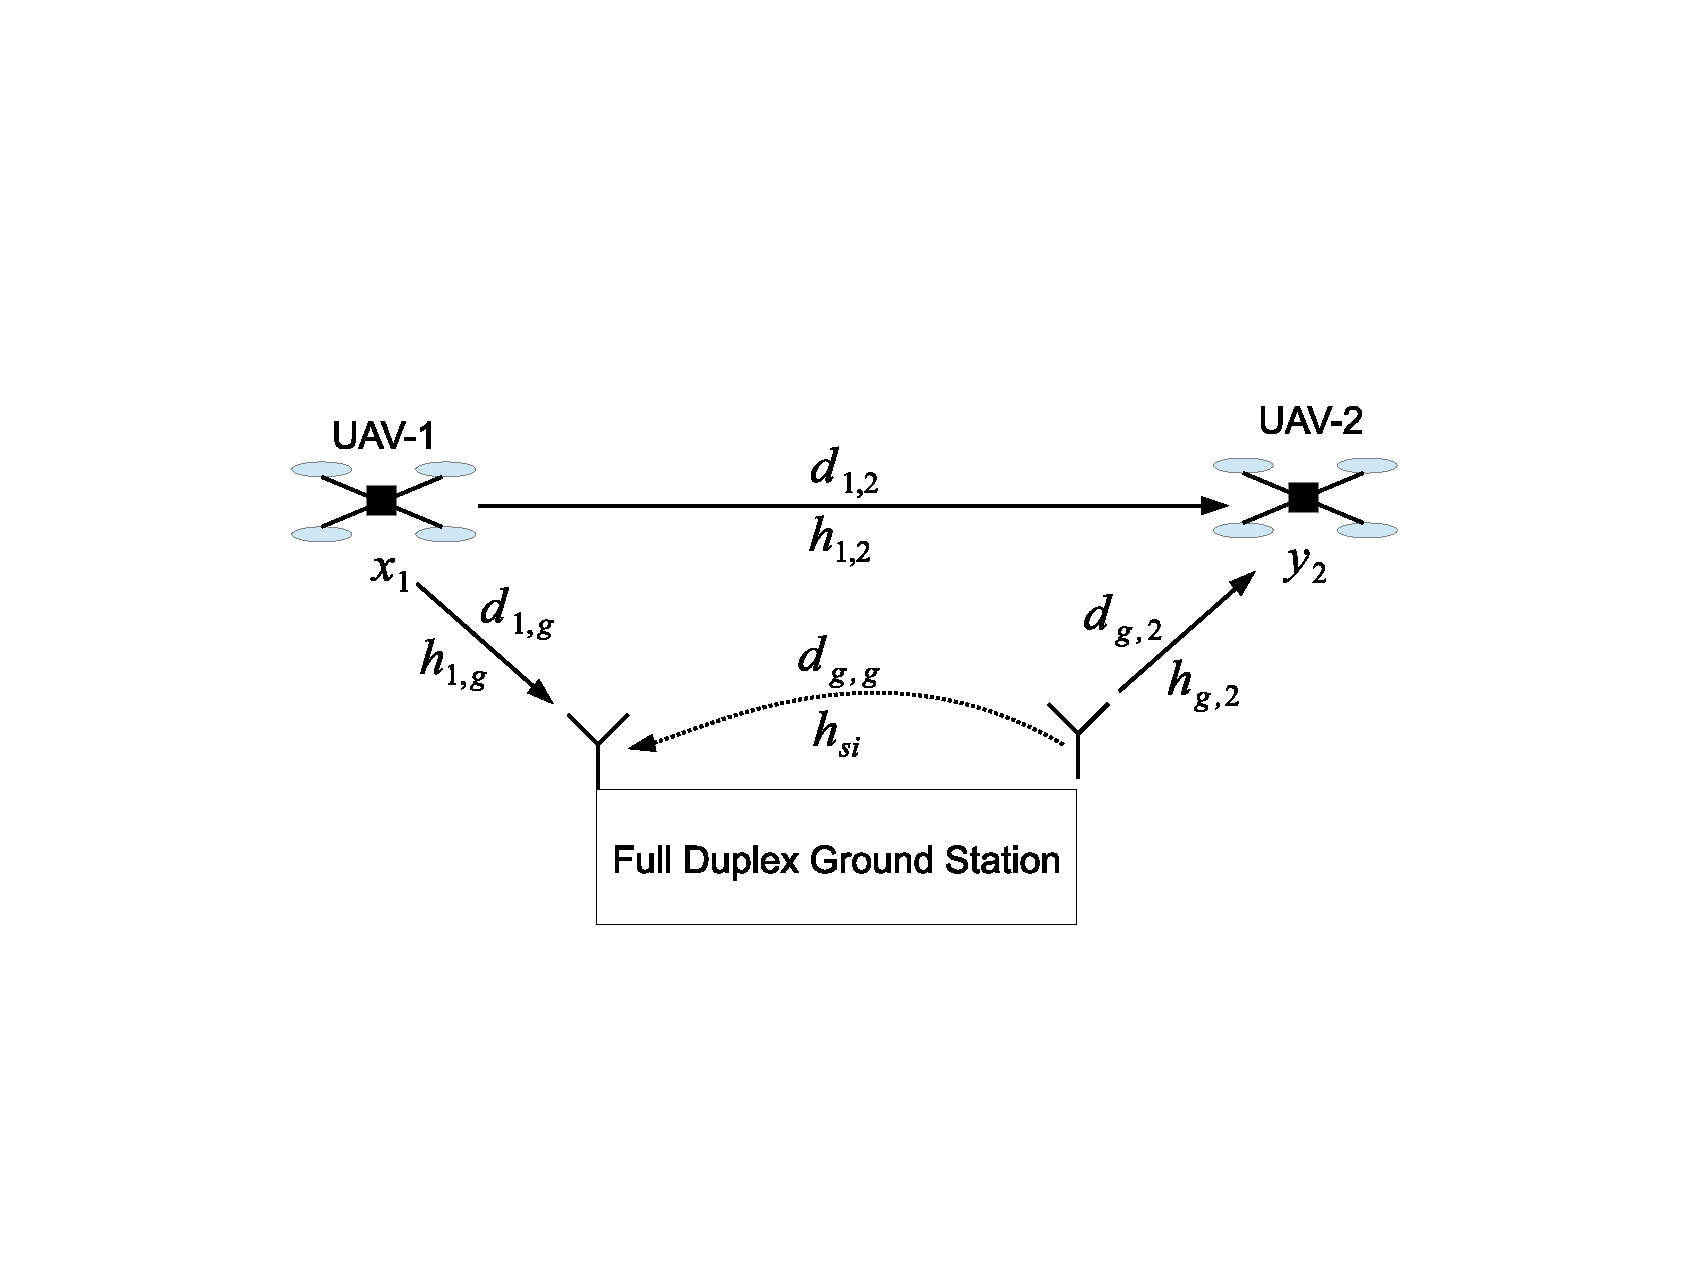
\includegraphics [width=0.8\columnwidth]{chap4_fig/block_diagram.eps} 
\vspace{-2.2cm}
\caption{Unmanned Aerial Vehicle 1 (UAV-1) and Unmanned Aerial Vehicle 2 (UAV-2) operating in HD mode while communicating with the FD GS.}
%\vspace{-0.5cm}
\label{fig:JD_HBD_UCS_1}
\end{figure}

Fig. \ref{fig:JD_HBD_UCS_1} shows the proposed HBD-UCS for UAV communications in a suburban environment between an FD-enabled GS node and two HD UAVs. \textcolor{black}{\footnote{\textcolor{black}{The present chapter can be extended to consider an arbitrary number of uplink and downlink UAVs. To enable the modeling and analysis of such a multi-UAV network, the signal model at the GS and downlink UAVs will need to be modified. Furthermore, stochastic geometry tools, i.e., the BPP model, will need to be employed to accurately model UAV deployment. These issues are addressed in Chapter \ref{chap:HBD_multi_UAV}, where new signal models that considers the BPP model are proposed for an HBD multi-UAV network.}}} In particular, Unmanned Aerial Vehicle 1 (UAV-1) transmits non-CNPC data to the GS while Unmanned Aerial Vehicle 2 (UAV-2) concurrently receives CNPC data from the GS on the same spectrum, e.g., L-band. Two antennas, one for transmission and another for reception of signals, with a shared local oscillator are assumed at the FD-enabled GS. Also, the Doppler effect as a result of UAV mobility is assumed to be compensated. Clearly, spectrum utilization is improved at the expense of introducing SI and inter-UAV interference at the FD-enabled GS and UAV-2, respectively. To enable realistic modeling of the suburban environment, Rician fading is assumed on all UAV communication channels \cite{matolak2017air_suburban}. Additionally, the SI signal is assumed to undergo passive SI mitigation before active SI mitigation at the FD-enabled GS. Thus, we consider only residual SI at the FD-enabled GS, with the SI link ($h_{si}$) modeled as a Rician fading channel to account for passive and active SI mitigation \cite{ahmed2015all}. A summary of important notations is also given in Table \ref{table:JD_HBD_UCS_summary_impt_notations}.

\subsection{Ground Station}
At the FD-enabled GS, let $x_{gs}[t]$ and $x_1[t]$ be the transmitted signals from GS and UAV-1, respectively, where the SOI and the SI signal are $x_1[t]$ and $x_{si}[t]=x_{gs}[t]$, respectively. Additionally, let $h_{1,g}[t]$ be the channel between UAV-1 and GS, and $h_{si}$ be the SI channel gain. Then, the received signal at GS can be written as \cite{sahai2013impact}:
%%%%%%%%%%%%%%%%%%%%%%%%%%%%%%%%%%%%%%%%%%%%%%%%%%%%%%%%%%%%%%%%%%%%%%%%%%%%%%%%%
\begin{eqnarray} \label{JD_HBD_UCS_y_gs}
y_{gs}[t] & = & \sqrt{\Omega_{X}}h_{1,g}[t]x_{1}[t] + \sqrt{\Omega_X\alpha_{g,g}}|h_{si}|\gamma_{\phi}w_{\phi}[t]  + \sqrt{\Omega_X\alpha_{g,g}} |\widetilde{h}_{si}|x_{si}[t] + w_{g}[t],
\end{eqnarray}
%%%%%%%%%%%%%%%%%%%%%%%%%%%%%%%%%%%%%%%%%%%%%%%%%%%%%%%%%%%%%%%%%%%%%%%%%%%%%%%%%
where $\widetilde{h}_{si}$ is the error of the imperfect SI channel gain estimate, defined as $\widetilde{h}_{si}=h_{si}-\widehat{h}_{si}$, and $\widehat{h}_{si}$ is the imperfect estimation of the SI channel gain. To model the worst case residual SI, the channel estimation error ($\widetilde{h}_{si}$) is modeled as a circularly symmetric zero-mean complex Gaussian random variable RV with variance $\epsilon$ \cite{zlatanov2017capacity}.

Additionally, let the AWGN at GS be $w_{g}[t]$, with zero-mean and variance $\sigma_g^2$, and let the phase noise term $w_{\phi}[t]$ follow a Gaussian distribution with zero-mean and unit variance, scaled by the strength of the phase noise $\gamma_{\phi}$ \footnote{The scaling factor $\gamma_{\phi}$ models the jitter present in oscillators due to hardware imperfections \cite{sahai2013impact}} \cite{sahai2013impact}. 


Let the average received signal power of the SOI, normalized with the GS receiver noise variance ($\sigma_g^2$), be $\Omega_{X}$, which is related to the transmit power $P_{t}$ (Watts) and distance $d_{1,g}$ (km) as:
%%%%%%%%%%%%%%%%%%%%%%%%%%%%%%%%%%%%%%%%%%%%%%%%%%%%%%%%%%%%%%%%%%%%%%%%%%%%%%%%%
\begin{eqnarray} \label{JD_HBD_UCS_Omega_x_soi}
\Omega_{X} \propto \frac{P_t}{\left(d_{1,g}\right)^{n}\sigma_g^2},
\end{eqnarray}
%%%%%%%%%%%%%%%%%%%%%%%%%%%%%%%%%%%%%%%%%%%%%%%%%%%%%%%%%%%%%%%%%%%%%%%%%%%%%%%%%
where $n$ is the pathloss exponent. We select the channel between UAV-1 and GS as the reference link, with the average received signal power in the other links expressed relative to the reference link to represent the inter-UAV interference level $\alpha_{i,j}$ as follows:
%%%%%%%%%%%%%%%%%%%%%%%%%%%%%%%%%%%%%%%%%%%%%%%%%%%%%%%%%%%%%%%%%%%%%%%%%%%%%%%%%
\begin{eqnarray} \label{JD_HBD_UCS_alpha_i_j}
\alpha_{i,j} = \bigg(\frac{d_{1,g}}{d_{i,j}}\bigg)^n, i\in\left\{g,1\right\}, j\in\left\{g,2\right\}.
\end{eqnarray}
%%%%%%%%%%%%%%%%%%%%%%%%%%%%%%%%%%%%%%%%%%%%%%%%%%%%%%%%%%%%%%%%%%%%%%%%%%%%%%%%%
From (\ref{JD_HBD_UCS_Omega_x_soi}) and (\ref{JD_HBD_UCS_alpha_i_j}), the average received SI power at GS can be expressed as $\Omega_X\alpha_{g,g}$. 

\subsection{Unmanned Aerial Vehicle 2}

The SOI and the interfering signal at UAV-2 are $x_{gs}[t]$ and $x_1[t]$, respectively. Let $h_{g,2}[t]$ be the channel between GS and UAV-2, and let $h_{1,2}[t]$ be the channel between UAV-1 and UAV-2. Let $w_{2}[t]$ be the AWGN at UAV-2 with zero-mean and variance $\sigma_2^2$. Then, the received signal at UAV-2 can be expressed as:
%%%%%%%%%%%%%%%%%%%%%%%%%%%%%%%%%%%%%%%%%%%%%%%%%%%%%%%%%%%%%%%%%%%%%%%%%%%%%%%%%
\begin{eqnarray} \label{JD_HBD_UCS_y_as2}
y_{2}[t] = \sqrt{\Omega_{X}\alpha_{g,2}}h_{g,2}[t]x_{gs}[t] + \sqrt{\Omega_{X}\alpha_{1,2}}h_{1,2}[t]x_{1}[t] +  w_{2}[t], 
\end{eqnarray}
%%%%%%%%%%%%%%%%%%%%%%%%%%%%%%%%%%%%%%%%%%%%%%%%%%%%%%%%%%%%%%%%%%%%%%%%%%%%%%%%%
where $\Omega_{X}\alpha_{g,2}$ and $\Omega_{X}\alpha_{1,2}$ indicate the average received signal powers of the SOI and interfering signal, respectively. 

As interference is present at UAV-2, we consider three approaches to handle the interference. The first approach is to assume an II detector at UAV-2 by treating $x_1[t]$ as noise, thus effectively ignoring interference. The second approach assumes a two-stage SIC detector at UAV-2 where $x_1[t]$ is detected and removed before $x_{gs}[t]$ is detected \cite{narasimhan2007individual}. The final approach assumes a joint detector where both $x_{gs}[t]$ and $x_1[t]$ are jointly detected \cite{blomer2009transmission}.

\begin{table}[]
\centering
\caption{Summary of Important Notations}
\label{table:JD_HBD_UCS_summary_impt_notations} 
\scalebox{0.8}{
\begin{tabular}{ll}
\hline
\textbf{Notations}		& \textbf{Description}																			\\  \hline \hline
$\Omega_X$						& Average received power																		\\
$\alpha_{i,j}, i\in\left\{g,1\right\}, j\in\left\{g,2\right\}, i \neq j$ & Strength of interference between $i$ and $j$				\\
$\epsilon$						& SI channel estimation error	at the FD-enabled GS					\\
$\gamma_{\phi}^2$			& Strength of phase noise at the FD- enabled GS oscillator	\\
$\sigma_g^2$					& Strength of AWGN at the FD-enabled GS											\\ 
$\sigma_2^2$					& Strength of AWGN at the UAV-2															\\ \hline
\end{tabular}}
\end{table}
%A summary of important notations is also given in Table \ref{table:JD_HBD_UCS_summary_impt_notations}.

%%%%%%%%%%%%%%%%%%%%%%%%%%%%%%%%%%%%%%%%%%%%%%%%%%%%%%%%%%%%%%%%%%%%%%%%%%%%%%%%%%%%%%%%%%%%%%%%%%%%%%%%%%%%%%%%%%%%%%%%%%%%%%%%%%%%%%%%%
% Section 3 : Outage Probability
\section{Outage Probability Derivations} \label{JD_HBD_UCS_subsec_UAV2_JD}
In this section, we derive the closed-form outage probability expression for the joint detector at UAV-2. As inter-UAV interference increases, we show that the outage probability of the joint detector approaches that of an interference-free UAV-2. We also define the system level outage probability, along with references for benchmark schemes, to identify bottlenecks in the proposed HBD-UCS system. 

\subsection{Joint Detector at UAV-2}
Let $R^{i}_{1}$ and $R^{i}_{gs}$ be the transmission rates of UAV-1 and GS, respectively, where $i \in \{HBD,HD\}$, and $R^{i}_{sum} = R^{i}_{1}+R^{i}_{gs}$ be the sum rate of the system. To maintain the same sum rate, the transmission rate of HD systems must be twice that of HBD systems as spectrum is shared between nodes in the former \cite{ahmed2015all,kwon2010optimal}. Thus, let $R_{j}^{HBD}=\frac{1}{2}R_{j}^{HD}$ for $ j \in \{1, gs\}$ to maintain a fair comparison between HBD-UCS and HD-UCS.

At UAV-2, let the instantaneous received signal power of the SOI and the inter-UAV interference be $X_{gs} = \Omega_{X}\alpha_{g,2}|h_{g,2}|^2$ and $Y_{1}=\Omega_{X}\alpha_{1,2}|h_{1,2}|^2$, respectively, where $X_{gs}$ and $Y_{1}$ are independent non-centered Chi-squared distributed RV with respective Rician $K$ factors $K_{X_{gs}}$ and $K_{Y_1}$.

\begin{figure} [tbp]
\centering
\vspace{-0.5cm}
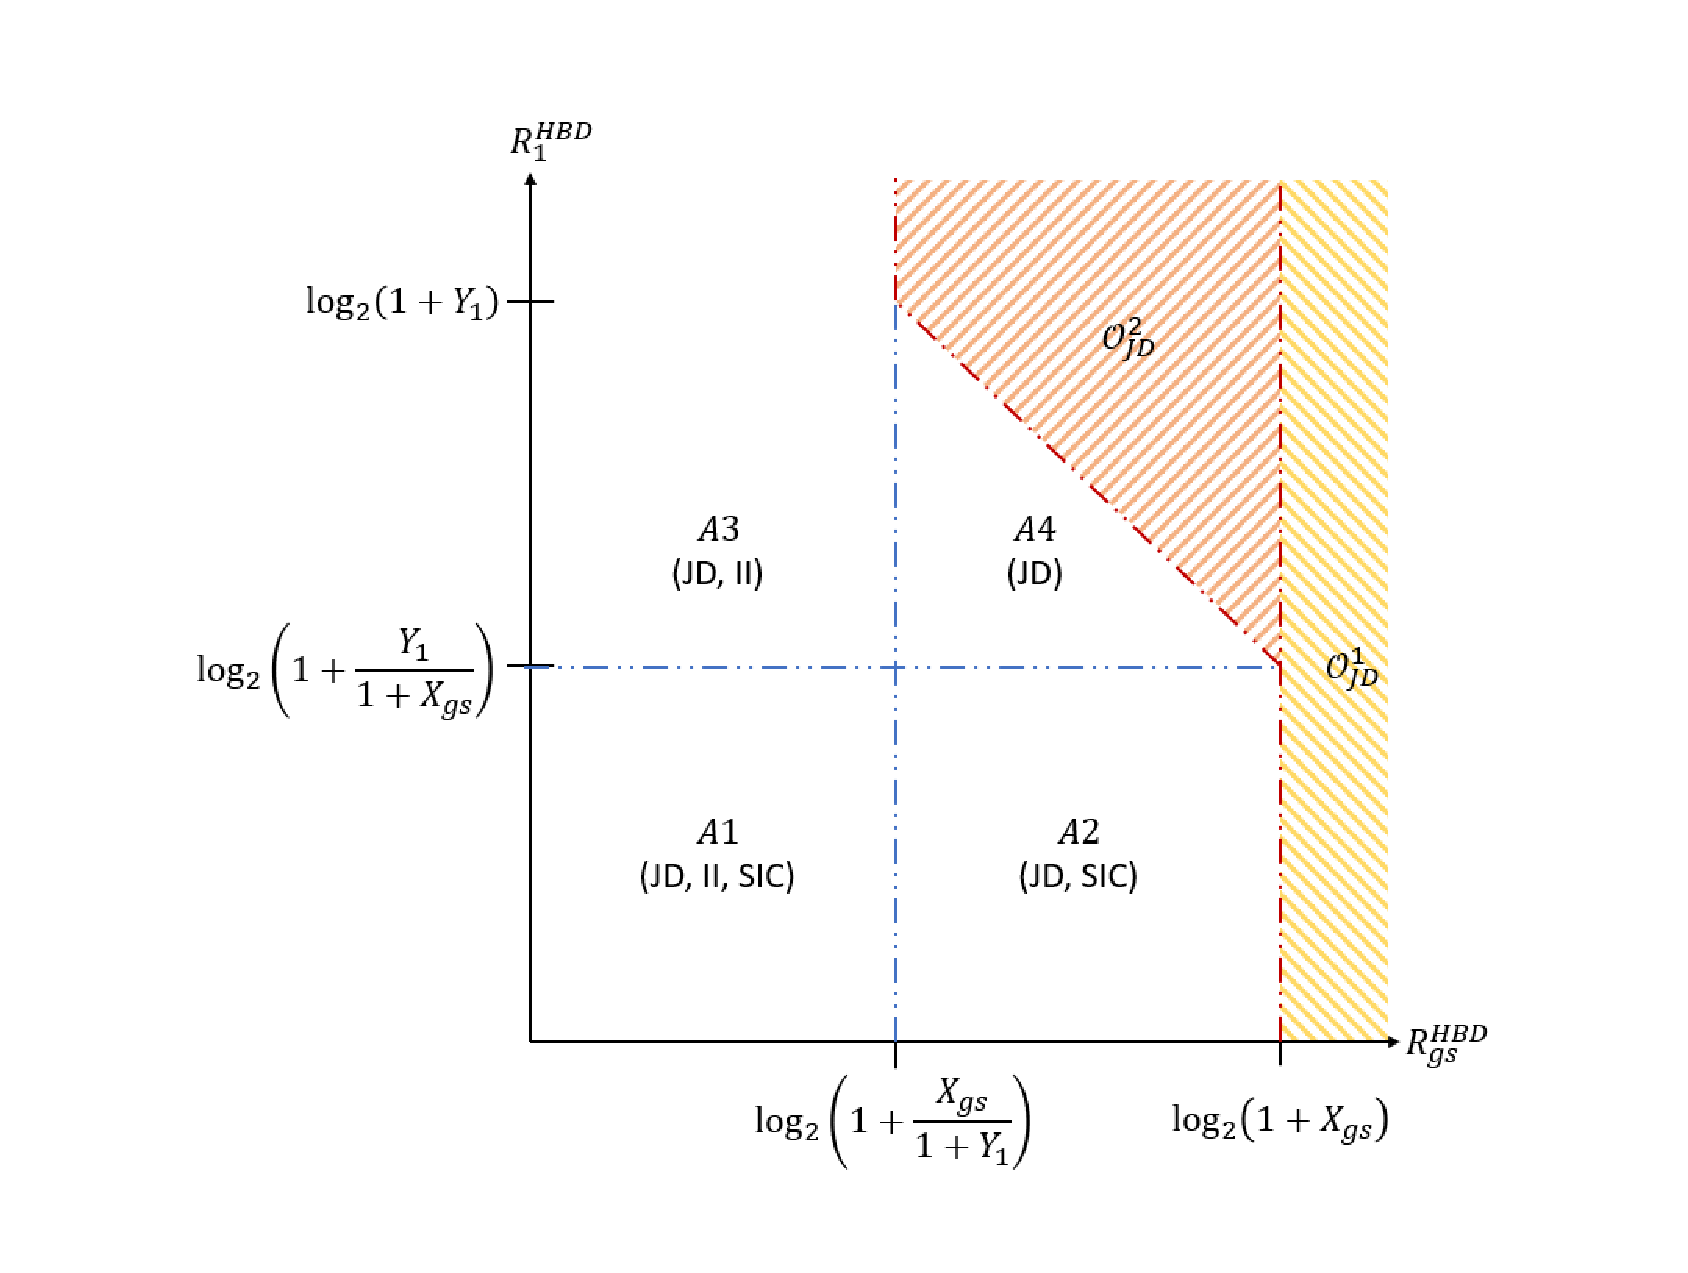
\includegraphics [width=0.6\columnwidth]{chap4_fig/rate_regions.eps} 
\vspace{-0.5cm}
\caption{The achievable instantaneous rate regions of the II, SIC and joint detectors (unshaded areas) at UAV-2 with respect to the transmission rates of the GS $\big(R_{GS}^{HBD}\big)$ and UAV-1 $\big(R_{1}^{HBD}\big)$. The shaded areas, $\mathcal{O}_{JD}^{1}$ and $\mathcal{O}_{JD}^{2}$, respectively denote the outage region of the joint detector if SOI detection fails or if the sum rate constraint is not met.}
\vspace{-0.25cm}
\label{fig:JD_HBD_UCS_rate_regions}
\end{figure}

To mitigate inter-UAV interference, the joint detector at UAV-2 simultaneously detects both SOI and interference from GS and UAV-1, respectively. The resultant instantaneous achievable rate region of the joint detector ($A1$ to $A4$), along with the II detector ($A1$ and $A3$) and the SIC detector ($A1$ and $A2$), are illustrated in Fig. \ref{fig:JD_HBD_UCS_rate_regions}. Based on the instantaneous achievable rate region, the HBD outage event of the joint detector at UAV-2 is defined as:
%%%%%%%%%%%%%%%%%%%%%%%%%%%%%%%%%%%%%%%%%%%%%%%%%%%%%%%%%%%%%%%%%%%%%%%%%%%%%%%%%
\begin{eqnarray}
							& \mathcal{O}_{2}^{HBD(JD)} & = \mathcal{O}_{JD}^{1} \cup \mathcal{O}_{JD}^{2} \label{JD_HBD_UCS_outage_JD_overall} \\
\text{where}	& \mathcal{O}_{JD}^{1} 			& = \bigg\{h_{g,2}, h_{1,2} : R_{gs}^{HBD} > \log_{2}\bigg(1+X_{gs}\bigg)\bigg\}, \label{JD_HBD_UCS_outage_JD_soi}\\
							& \mathcal{O}_{JD}^{2} 			& = \bigg\{h_{g,2}, h_{1,2} : R_{1}^{HBD} + R_{gs}^{HBD} > \log_{2}\bigg(1+X_{gs}+Y_{1} \bigg), \nonumber\\
							&														& \hspace{0.5cm} \log_{2}\bigg(1+\frac{X_{gs}}{1+Y_{1}} \bigg) \leq R_{gs}^{HBD} \hspace{-0.05cm} \leq \hspace{-0.05cm} \log_{2}\bigg(1+X_{gs}\bigg) \bigg\} \label{JD_HBD_UCS_outage_JD_int}.
\end{eqnarray}
%%%%%%%%%%%%%%%%%%%%%%%%%%%%%%%%%%%%%%%%%%%%%%%%%%%%%%%%%%%%%%%%%%%%%%%%%%%%%%%%%
\begin{remark} \label{remark_jd}
\textit{The joint detector outage event $\big(\mathcal{O}_{2}^{HBD(JD)}\big)$ occurs if SOI detection fails $\big(\mathcal{O}_{JD}^{1}\big)$ or if the sum rate constraint is not met $\big(\mathcal{O}_{JD}^{2}\big)$. Evidently, meeting the sum rate constraint $\big(\mathcal{O}_{JD}^{2}\big)$ enables the joint detector to attain a larger rate region than the II and the SIC detectors at the cost of complex hardware \cite{shubhi2017joint,blomer2009transmission}.}
\end{remark}

In a two-user multiple access channel, the joint detector simultaneously decodes the two user's data streams as the SOIs. An outage event occurs if either of the streams cannot be decoded \cite{narasimhan2007individual}. In contrast, only the signal from the FD-enabled GS is treated as the SOI while the signal from UAV-2 is treated as interference in this chapter. Therefore, the joint detector tries to decode only the SOI, while utilizing the structure of the interfering signal. Consequently, the interfering signal can be transmitted at a higher rate than the capacity of the interfering link \cite{bennatan2014soft}.

The advantages of the joint detector in this chapter is evident in Fig. \ref{fig:JD_HBD_UCS_rate_regions}. In particular, (\ref{JD_HBD_UCS_outage_JD_soi}) and (\ref{JD_HBD_UCS_outage_JD_int}) are obtained using the above principles. A similar decoding algorithm for an interference-limited receiver in a two-user interference channel is also investigated in \cite{bandemer2012simultaneous,nam2014advanced}, where similar achievable instantaneous rate regions were obtained. For the II and SIC detectors, the respective achievable instantaneous rate regions are obtained using the outage events definition in \cite{ernest2019outage}. Together, the achievable instantaneous rate regions in Fig. \ref{fig:JD_HBD_UCS_rate_regions} form the basis for Remark \ref{remark_jd}.

Next, let $\overline{\alpha}\big(q,\Omega,K,\gamma\big)$ be the CDF expansion of a Rician fading channel, which is defined as:
%%%%%%%%%%%%%%%%%%%%%%%%%%%%%%%%%%%%%%%%%%%%%%%%%%%%%%%%%%%%%%%%%%%%%%%%%%%%%%%%%
\begin{eqnarray} \label{JD_HBD_UCS_alpha_func}
\overline{\alpha}\big(q,\Omega,K,\gamma\big) = (-1)^q \exp(-K) \frac{{L_q}^{(0)}(K)}{(1+q)!} \Bigg(\frac{(1+K)}{\Omega}\gamma\Bigg)^{q+1},
\end{eqnarray}
%%%%%%%%%%%%%%%%%%%%%%%%%%%%%%%%%%%%%%%%%%%%%%%%%%%%%%%%%%%%%%%%%%%%%%%%%%%%%%%%%
where $q$, $\Omega$, $K$ and $\gamma$ represents an arbitrary non-negative integer, average received power of a Rician signal, Rician $K$ factor and threshold, respectively, and ${L_q}^{(0)}(\bullet)$ represents the $q$-th degree, zero-order Laguerre polynomials \cite{andras2011generalized}. Then, the closed-form outage probability expression for the joint detector is presented in the following theorem.

\begin{theorem}
The closed-form expression for the outage probability with joint detector at UAV-2 is:
%%%%%%%%%%%%%%%%%%%%%%%%%%%%%%%%%%%%%%%%%%%%%%%%%%%%%%%%%%%%%%%%%%%%%%%%%%%%%%%%%
\begin{eqnarray} \label{JD_HBD_UCS_P_out_as2_JD}
Pr\big(\mathcal{O}_{2}^{HBD(JD)}\big) & \approx & 1 - Q_1\left( \sqrt{2K_{X_{gs}}}, \sqrt{\frac{2(K_{X_{gs}}+1)\gamma_{th,2}^{HBD}}{\Omega_{X}\alpha_{g,2}}} \right) \nonumber\\
& & \hspace{0cm} + \sum_{n=0}^{K_{tr}} \hspace{-0.05cm} \sum_{i=0}^{n} \hspace{-0.05cm} \sum_{j=0}^{i+1} \overline{\alpha}(i,\Omega_X\alpha_{1,2},K_{Y_1},1) \overline{\alpha}(n-i,\Omega_X\alpha_{g,2},K_{X_{gs}},1) \binom{i+1}{j} \nonumber\\
& & \hspace{1cm} \times (-1)^{i+1} G_1\big(i,j,b_2,\gamma_{th,2}^{HBD}\big) \frac{G_2\big(j+n-i+1,b_1,\gamma_{th,2}^{HBD}\big)}{j+n-i+1},
\end{eqnarray}
%%%%%%%%%%%%%%%%%%%%%%%%%%%%%%%%%%%%%%%%%%%%%%%%%%%%%%%%%%%%%%%%%%%%%%%%%%%%%%%%%
where $K_{tr}$ is the truncation order, $\gamma_{th,2}^{HBD} = 2^{R_{gs}^{HBD}}-1$ is the threshold, $b_1 = 2^{R_{1}^{HBD}}(2^{R_{gs}^{HBD}}-1)$, $b_2 = 2^{R_{1}^{HBD}+R_{gs}^{HBD}}-1$, $G_1\big(i,j,b_2,\gamma_{th,2}^{HBD}\big)=(-b_2)^{i+1-j} - (-\gamma_{th,2}^{HBD})^{-j}$, $G_2\big(j+n-i+1,b_1,\gamma_{th,2}^{HBD}\big) = (b_1)^{j+n-i+1} - (\gamma_{th,2}^{HBD})^{j+n-i+1}$ and $Q_1\left(\cdot,\cdot\right)$ is the Marcum Q function \cite{andras2011generalized}
\end{theorem}
\begin{proof}
The proof can be found in Appendix \ref{JD_HBD_UCS_JD_proof}.
\end{proof}

\begin{remark}
\textit{The first two terms on the RHS of (\ref{JD_HBD_UCS_P_out_as2_JD}) are due to the outage event $\mathcal{O}_{JD}^{1}$. These two terms also correspond to the outage probability of an interference-free UAV-2. The third term on the RHS of (\ref{JD_HBD_UCS_P_out_as2_JD}) is due to the outage event $\mathcal{O}_{JD}^{2}$, where the functions $\overline{\alpha}(i,\Omega_X\alpha_{1,2},K_{Y_1},1)$ and $\overline{\alpha}(n-i,\Omega_X\alpha_{g,2},K_{X_{gs}},1)$ are due to the inter-UAV interference and SOI, respectively. From (\ref{JD_HBD_UCS_P_out_as2_JD}), it is evident that failure to either detect the SOI or meet the sum rate constraint contributes to outage probability.}
\end{remark}

The expression in (\ref{JD_HBD_UCS_P_out_as2_JD}) is only valid if the power series in the second term on the RHS converges, which is proven in the following theorem.
\begin{theorem}
The power series in (\ref{JD_HBD_UCS_P_out_as2_JD}) has a convergence radius of $\infty$.
\end{theorem}
\begin{proof}
The proof can be found in Appendix \ref{JD_HBD_UCS_JD_convg_proof}.
\end{proof}

It should be noted that the differentiation of a convergent power series, e.g., (\ref{JD_HBD_UCS_appdx_JD_9}), is also valid within the convergence radius \cite{amann2005analysis,gradshteyn2014table}, which is useful for deriving expressions related to finite SNR analysis in the next section.

It is known that the joint detector is effective when strong interference is encountered \cite{zahavi2017cooperation,zhou2015mac,shubhi2017joint,blomer2009transmission}. To investigate the effect of strong inter-UAV interference, we evaluate the limit of $\overline{\alpha}(i,\Omega_X\alpha_{1,2},K_{Y_1},1)$ with respect to $\alpha_{1,2}$. In particular, we evaluate the limit for the extreme case of very strong inter-UAV interference ($\alpha_{1,2} \to \infty$), using the same approach in \cite[eq.(11)]{ernest2019outage}. From (\ref{JD_HBD_UCS_alpha_func}) and (\ref{JD_HBD_UCS_P_out_as2_JD}), it can be seen that the outage probability with joint detector approaches that of an interference-free UAV-2 as $\alpha_{1,2} \to \infty$. Hence, the joint detector is suitable for strong interference scenarios since the detection of the SOI becomes easier. Although the SIC is also known to perform well at very strong inter-UAV interference levels, the joint detector still outperforms the SIC detector at high SNRs, as will be shown in Section \ref{JD_HBD_UCS_num_results_sec}. More importantly, (\ref{JD_HBD_UCS_P_out_as2_JD}) also suggests the possibility of the joint detector attaining near-genie-aided (\textcolor{black}{near perfect}), i.e., interference-free, outage performance when interference is sufficiently strong.

\subsection{Benchmark Schemes and System Level Outage Probability} \label{JD_HBD_UCS_sub_sec_ref_schemes_outage}

\begin{table}[]
\centering
\caption{References for the outage probability of the benchmark schemes}
\label{table:JD_HBD_UCS_ref_schemes_outage}
\scalebox{0.7}{\begin{tabular}{ccc}
\hline 
Protocol/Detector						& Notation 																	& Reference \\ \hline \hline \vspace{0.05cm}
II Detector at GS			&	$Pr\big(\mathcal{O}_{gs}^{HBD}\big)$			& \cite[eq. (6)]{ernest2019outage}  \\ \vspace{0.05cm}
II Detector at UAV-2 	& $Pr\big(\mathcal{O}_{2}^{HBD(II)}\big)$ 	& \cite[eq. (8)]{ernest2019outage} \\ \vspace{0.05cm} 
SIC Detector at UAV-2	&	$Pr\big(\mathcal{O}_{2}^{HBD(SIC)}\big)$	& \cite[eq. (10)]{ernest2019outage}  \\ \vspace{0.05cm}
HD-UCS at GS					&	$Pr\big(\mathcal{O}_{gs}^{HD}\big)$				& \cite[eq. (12)]{ernest2019outage}  \\ \vspace{0.05cm}
HD-UCS at UAV-2				&	$Pr\big(\mathcal{O}_{2}^{HD}\big)$				& \cite[eq. (13)]{ernest2019outage}  \\ \hline
\end{tabular}} \vspace{-0.5cm}
\end{table}


In this chapter, the II detector, SIC detector, and the HD-UCS are also considered at UAV-2. These schemes are treated as benchmark schemes as the associated outage probability expressions are already available in the literature, with the references provided in Table \ref{table:JD_HBD_UCS_ref_schemes_outage}. At the GS, residual SI is present and thus, the GS effectively adopts an II detector. The outage probability expression for the GS is also available in the literature and is similarly provided in Table \ref{table:JD_HBD_UCS_ref_schemes_outage}.

To compare the overall performance of the HBD-UCS against the HD-UCS at the system level, we define the HBD and HD system level outage probability as:
\begin{eqnarray}
P_{out,system}^{\beta} & = & \max\big\{Pr\big(\mathcal{O}_{gs}^{HBD}\big),Pr\big(\mathcal{O}_{2}^{\beta}\big)\big\}, \\
P_{out,system}^{HD} & = & \max\big\{Pr\big(\mathcal{O}_{gs}^{HD}\big),Pr\big(\mathcal{O}_{2}^{HD}\big)\big\}
\end{eqnarray}
where $\beta \in \{HBD(II), HBD(SIC), HBD(JD)\}$. The defined HBD system level outage probability enables the identification of performance bottleneck in the proposed HBD-UCS.

% Section: Finite SNR Diversity Gain
\section{Finite SNR Analysis}

In this section, the necessary mathematical analysis and closed-form expressions for finite SNR diversity gains are presented for both fixed and variable transmission rate systems, with detailed derivations omitted for brevity.
%%%%%%%%%%%%%%%%%%%%%%%%%%%%%%%%%%%%%%%%%%%%%%%%%%%%%%%%%%%%%%%%%%%%%%%%%%%%%%%%%%%%%%%%%%%%%%%%%%%%%%%%%%%%%%%%%%%%%%%%%%%%%%%%%%%%%%%%%
\subsection{Finite SNR Diversity Gain}

The asymptotic diversity gain of a system, given by Zheng and Tse \cite[eq. (3)]{zheng2003diversity}, quantifies the outage probability decay rate at high SNR. However, the definition in \cite[eq. (3)]{zheng2003diversity} may not be accurate at low to moderate SNR ranges \cite{shin2008diversity}. 

To this end, finite SNR diversity gain definitions for low to moderate SNR ranges have been presented by Narasimhan \cite[eq. (5)]{narasimhan2006finite} and Shin et al. \cite{shin2008diversity}. Let $\mathcal{O}$, $Pr\big(\mathcal{O}\big)$, $R$, $\gamma$ and $\Omega$ be the outage event, outage probability, transmission rate, threshold and average received power with unit noise variance, respectively. Then, the finite SNR diversity gain ($d_f$) of a given system is \cite[eq. (5)]{narasimhan2006finite}:
%%%%%%%%%%%%%%%%%%%%%%%%%%%%%%%%%%%%%%%%%%%%%%%%%%%%%%%%%%%%%%%%%%%%%%%%%%%%%%%%%
\begin{eqnarray} \label{JD_HBD_UCS_df}
d_f = \frac{-\Omega}{Pr\big(\mathcal{O}\big)}\frac{\partial}{\partial\Omega}Pr\big(\mathcal{O}\big).
\end{eqnarray}
%%%%%%%%%%%%%%%%%%%%%%%%%%%%%%%%%%%%%%%%%%%%%%%%%%%%%%%%%%%%%%%%%%%%%%%%%%%%%%%%%

At high SNR, (\ref{JD_HBD_UCS_df}) is consistent with the asymptotic diversity gain definition given by Zheng and Tse \cite{zheng2003diversity}, as proven by Shin et al. \cite{shin2008diversity} and Heidarpour et al. \cite{heidarpour2017finite}. Moreover, (\ref{JD_HBD_UCS_df}) enables system designers to investigate the impact of residual SI and inter-UAV interference in HBD-UCS and to quantify potential outage performance improvements through code designs for the II, SIC and joint detectors at typical operating SNR ranges. 

\subsection{Finite SNR DMT Parameters}
For variable transmission rate systems, i.e., adaptive rate systems, the finite SNR multiplexing gain $r_f$ is defined as \cite[eq. (4)]{narasimhan2006finite}:
%%%%%%%%%%%%%%%%%%%%%%%%%%%%%%%%%%%%%%%%%%%%%%%%%%%%%%%%%%%%%%%%%%%%%%%%%%%%%%%%%
\begin{eqnarray} \label{JD_HBD_UCS_rf}
r_f = \frac{R(\Omega)}{\log_2(1+\Omega)}.
\end{eqnarray}
%%%%%%%%%%%%%%%%%%%%%%%%%%%%%%%%%%%%%%%%%%%%%%%%%%%%%%%%%%%%%%%%%%%%%%%%%%%%%%%%%

In variable transmission rate systems, $Pr\big(\mathcal{O}\big)$ is computed with respect to $\gamma=(1+\Omega)^{r_f}-1$. The finite SNR multiplexing gain indicates the sensitivity of $\gamma$ when $\Omega$ changes, and similar to (\ref{JD_HBD_UCS_df}), (\ref{JD_HBD_UCS_rf}) has also been proven by Shin et al. \cite{shin2008diversity} and Heidarpour et al. \cite{heidarpour2017finite} to be consistent with asymptotic multiplexing gain in \cite[eq. (3)]{zheng2003diversity}.

Let $\Delta(\Omega)=\widehat{\Omega}-\Omega$ where $\widehat{\Omega}>\Omega$. Then, extending upon (\ref{JD_HBD_UCS_df}), the finite SNR diversity gain for variable transmission rate systems (denoted as $d_{f}^{*}$) is \cite[eq. (36)]{shin2008diversity}:
%%%%%%%%%%%%%%%%%%%%%%%%%%%%%%%%%%%%%%%%%%%%%%%%%%%%%%%%%%%%%%%%%%%%%%%%%%%%%%%%%
\begin{eqnarray}
d_f^* & = & \frac{-\Omega}{Pr\big(\mathcal{O}\big)} \lim_{\Delta(\Omega)\to0} \Big[\frac{Pr\big(\mathcal{\widehat{O}}\big) - Pr\big(\mathcal{O}\big)}{\Delta(\Omega)}\Big] \label{JD_HBD_UCS_df_var_rate1} \\
& = & \frac{-\Omega}{Pr\big(\mathcal{O}\big)} \frac{\partial}{\partial\Delta(\Omega)} Pr\big(\mathcal{\widehat{O}}\big) \bigg|_{\Delta(\Omega)=0,} \label{JD_HBD_UCS_df_var_rate2}
\end{eqnarray}
%%%%%%%%%%%%%%%%%%%%%%%%%%%%%%%%%%%%%%%%%%%%%%%%%%%%%%%%%%%%%%%%%%%%%%%%%%%%%%%%%
where (\ref{JD_HBD_UCS_df_var_rate2}) is obtained from (\ref{JD_HBD_UCS_df_var_rate1}) by applying L'hopital's rule with respect to $\Delta(\Omega)$, $\mathcal{\widehat{O}}$ is the outage event with respect to $R\big(\Omega+\Delta(\Omega)\big)$ and $Pr\big(\mathcal{\widehat{O}}\big)$ is the outage probability with average received power $\widehat{\Omega}=\Omega+\Delta(\Omega)$, threshold $\widehat{\gamma}=[1+\Omega+\Delta(\Omega)]^{r_f}-1$ and $Pr\big(\mathcal{\widehat{O}}\big)=Pr\big(\mathcal{O}\big)$ when $\Delta(\Omega)=0$. Furthermore, although not explicitly shown in (\ref{JD_HBD_UCS_df_var_rate2}), we define $d_f^*$ to be non-negative, i.e., $d_f^* = \max\bigg\{0, \frac{-\Omega}{Pr\big(\mathcal{O}\big)} \frac{\partial}{\partial\Delta(\Omega)} Pr\big(\mathcal{\widehat{O}}\big) \bigg|_{\Delta(\Omega)=0} \bigg\}$, as it is a measure of the negative slope of the outage probability curve \cite{narasimhan2006finite}.

Let the normalized $n^{th}$ moment of a RV $Z$ be:
%%%%%%%%%%%%%%%%%%%%%%%%%%%%%%%%%%%%%%%%%%%%%%%%%%%%%%%%%%%%%%%%%%%%%%%%%%%%%%%%%
\begin{eqnarray} \label{JD_HBD_UCS_norm_moment}
M\{Z^{n}\}=\frac{E\{Z^{n}\}}{(\Omega)^{n}}
\end{eqnarray}
%%%%%%%%%%%%%%%%%%%%%%%%%%%%%%%%%%%%%%%%%%%%%%%%%%%%%%%%%%%%%%%%%%%%%%%%%%%%%%%%%
and let function $g(i,j,\Omega,r_f)$ be:
%%%%%%%%%%%%%%%%%%%%%%%%%%%%%%%%%%%%%%%%%%%%%%%%%%%%%%%%%%%%%%%%%%%%%%%%%%%%%%%%%
\begin{eqnarray} \label{JD_HBD_UCS_g_func}
g(i,j,\Omega,r_f) & = & \big([1 + \Omega]^{r_f}-1\big)^{i} (\Omega)^{j} \Big[ \big([1 + \Omega]^{r_f} - 1\big) \frac{j}{\Omega} + (i+1)(r_f)(1 + \Omega)^{r_f-1} \Big], \nonumber \\
\end{eqnarray}
%%%%%%%%%%%%%%%%%%%%%%%%%%%%%%%%%%%%%%%%%%%%%%%%%%%%%%%%%%%%%%%%%%%%%%%%%%%%%%%%%
where $i$ and $j$ are integers. The function $g(i,j,\Omega,r_f)$ reflects the outage probability decay rate of a variable transmission rate scheme due to average received power ($\Omega$) and finite SNR multiplexing gain ($r_f$) \cite{ernest2019outage}.

It should be noted that the resultant finite SNR diversity gain expression in (\ref{JD_HBD_UCS_df_var_rate2}) is based on \cite[eq. (36)]{shin2008diversity} and \cite[eq. (5)]{narasimhan2006finite}. Although \cite[eq. (36)]{shin2008diversity} and \cite[eq. (5)]{narasimhan2006finite} evaluated finite SNR diversity gain through different approaches and definitions, the former is based on the latter. Hence, (\ref{JD_HBD_UCS_df_var_rate2}) shows that both works are unified under the same principles. Similar to (\ref{JD_HBD_UCS_df}), the impact of residual SI and inter-UAV interference in adaptive HBD-UCS can be analyzed through (\ref{JD_HBD_UCS_df_var_rate2}).

%%%%%%%%%%%%%%%%%%%%%%%%%%%%%%%%%%%%%%%%%%%%%%%%%%%%%%%%%%%%%%%%%%%%%%%%%%%%%%%%%%%%%%%%%%%%%%%%%%%%%%%%%%%%%%%%%%%%%%%%%%%%%%%%%%%%%%%%
\subsection{Finite SNR Diversity Gain and DMT for HBD Systems}

For the joint detector, the finite SNR diversity gain ($d_{f,2}^{HBD(JD)}$) is given in the following proposition.
\begin{proposition} 
The finite SNR diversity gain at UAV-2 for the joint detector is:
%%%%%%%%%%%%%%%%%%%%%%%%%%%%%%%%%%%%%%%%%%%%%%%%%%%%%%%%%%%%%%%%%%%%%%%%%%%%%%%%%
\begin{eqnarray} \label{JD_HBD_UCS_df_fixed_UAV2_JD}
d_{f,2}^{HBD(JD)} & \approx & \frac{-\Omega_X}{Pr\big(\mathcal{O}_{2}^{HBD(JD)}\big)} \Bigg[ \sum_{m=0}^{K_{tr}} \overline{\alpha}\big(m,\alpha_{g,2},K_{X_{gs}},\gamma_{th,2}^{HBD}\big) \nonumber\\
& & \hspace{-0cm} \times (-m-1) (\Omega_{X})^{-m-2} + \sum_{n=0}^{K_{tr}}\sum_{i=0}^{n}\sum_{j=0}^{i+1} \overline{\alpha}(i,\alpha_{1,2},K_{Y_1},1) \nonumber\\
& & \hspace{-0cm} \times \overline{\alpha}(n-i,\alpha_{g,2},K_{X_{gs}},1) \binom{i+1}{j}(-1)^{i+1} G_1\big(i,j,b_2,\gamma_{th,2}^{HBD}\big) \nonumber\\
& & \hspace{-0cm} \times \frac{G_2\big(j+n-i+1,b_1,\gamma_{th,2}^{HBD}\big)}{j+n-i+1} (-n-2)(\Omega_X)^{-n-3} \Bigg].
\end{eqnarray}
%%%%%%%%%%%%%%%%%%%%%%%%%%%%%%%%%%%%%%%%%%%%%%%%%%%%%%%%%%%%%%%%%%%%%%%%%%%%%%%%%
\end{proposition}
\begin{proof}
At UAV-2, $d_{f,2}^{HBD(JD)}$ can be obtained from (\ref{JD_HBD_UCS_P_out_as2_JD}) and (\ref{JD_HBD_UCS_df}).
\end{proof}

The expression in (\ref{JD_HBD_UCS_df_fixed_UAV2_JD}) is accurate even at low to moderate $\Omega_X$, and it is useful in evaluating the impact of inter-UAV interference on outage probability decay trends. \textcolor{black}{\footnote{\textcolor{black}{To analytically gauge the accuracy of the new power series expressions presented in this Chapter, one will need to conduct a truncation analysis. Work in this direction is left as an open research challenge which can be addressed in future studies.}}} To uncover the asymptotic outage behavior for the joint detector, we evaluate (\ref{JD_HBD_UCS_df_fixed_UAV2_JD}) at high $\Omega_X$, as shown in the following corollary.

\begin{corollary} \label{JD_HBD_UCS_asymptotic_JD}
At UAV-2, the joint detector achieves full diversity at high SNR regimes.
\begin{proof}
To prove Corollary \ref{JD_HBD_UCS_asymptotic_JD}, we have to show that 
\begin{eqnarray} \label{JD_HBD_UCS_asymp_df_fixed_UAV2_JD}
\lim_{\Omega_X\to\infty} \frac{-\Omega_X}{Pr\big(\mathcal{O}_{2}^{HBD(JD)}\big)} \frac{\partial}{\partial\Omega_X}Pr\big(\mathcal{O}_{2}^{HBD(JD)}\big) & = & 1.
\end{eqnarray}

By simplifying (\ref{JD_HBD_UCS_df_fixed_UAV2_JD}) and evaluating the limits with respect to $\Omega_X$ leads to the following expression:
%%%%%%%%%%%%%%%%%%%%%%%%%%%%%%%%%%%%%%%%%%%%%%%%%%%%%%%%%%%%%%%%%%%%%%%%%%%%%%%%%
\begin{eqnarray} \label{JD_HBD_UCS_df_fixed_UAV2_JD_2}
\lim_{\Omega_X\to\infty} d_{f,2}^{HBD(JD)} & \approx & \lim_{\Omega_X\to\infty} \frac{-1}{\Omega_X \cdot Pr\big(\mathcal{O}_{2}^{HBD(JD)}\big)} \Bigg[ \sum_{m=0}^{K_{tr}} \overline{\alpha}\big(m,\alpha_{g,2},K_{X_{gs}},\gamma_{th,2}^{HBD}\big) (-m-1) (\Omega_{X})^{-m} \nonumber\\
& & \hspace{-0cm} + \sum_{n=0}^{K_{tr}}\sum_{i=0}^{n}\sum_{j=0}^{i+1} \overline{\alpha}(i,\alpha_{1,2},K_{Y_1},1) \overline{\alpha}(n-i,\alpha_{g,2},K_{X_{gs}},1) \binom{i+1}{j} \nonumber\\
& & \hspace{1cm} \times G_1\big(i,j,b_2,\gamma_{th,2}^{HBD}\big) \frac{G_2\big(j+n-i+1,b_1,\gamma_{th,2}^{HBD}\big) (-n-2)}{(-1)^{-i-1}(j+n-i+1)(\Omega_X)^{n+1}} \Bigg].
\end{eqnarray}
%%%%%%%%%%%%%%%%%%%%%%%%%%%%%%%%%%%%%%%%%%%%%%%%%%%%%%%%%%%%%%%%%%%%%%%%%%%%%%%%%

For the first term in the numerator of (\ref{JD_HBD_UCS_df_fixed_UAV2_JD_2}), $\lim_{\Omega_X\to\infty} \left(\Omega_X\right)^{-m} = 0$ when $m>0$ and $\lim_{\Omega_X\to\infty} \left(\Omega_X\right)^{-m} = 1$ when $m=0$. Likewise for the second term in the numerator, $\lim_{\Omega_X\to\infty} \left(\Omega_X\right)^{-n-1} = 0$ for $n\geq0$. Therefore, we only consider $m=0$ when evaluating the limit in the numerator. Repeating the same steps for the denominator in (\ref{JD_HBD_UCS_df_fixed_UAV2_JD_2}) leads to (\ref{JD_HBD_UCS_asymp_df_fixed_UAV2_JD})
\end{proof}
\end{corollary}

From (\ref{JD_HBD_UCS_asymp_df_fixed_UAV2_JD}), the joint detector's diversity gain is better than the II and SIC detectors, as shown in \cite[eq. (28)]{ernest2019outage}, and is equivalent to an HD-UCS \cite[eq. (31)]{ernest2019outage}.

For the GS and UAV-2 operating under a variable rate transmission scheme, let the variable transmission rate of UAV-1 and GS be $R_1^{HBD}(\Omega_X)=r_{f,1}\log_2(1+\Omega_X)$ and $R_{gs}^{HBD}(\Omega_X)=r_{f,gs}\log_2(1+\Omega_X)$, respectively. Also, let the threshold at GS and UAV-2 be $\gamma_{th,gs}^{HBD} = [1+\Omega_X]^{r_{f,1}}-1$ and $\gamma_{th,2}^{HBD} = [1+\Omega_X]^{r_{f,gs}}-1$, respectively. Then, the variable rate finite SNR diversity gain expressions are presented in the following propositions.
\begin{proposition}
At GS, the variable rate finite SNR diversity gain is:
%%%%%%%%%%%%%%%%%%%%%%%%%%%%%%%%%%%%%%%%%%%%%%%%%%%%%%%%%%%%%%%%%%%%%%%%%%%%%%%%%
\begin{eqnarray} \label{JD_HBD_UCS_df_var_gs}
d_{f,gs}^{HBD*} & \approx & \frac{-\Omega_X}{Pr\big(\mathcal{O}_{gs}^{HBD}\big)} \sum_{q=0}^{K_{tr}}\sum_{l_1+l_2+l_3=q+1} \overline{\alpha}\big(q,1,K_{X_1},1\big) \frac{(q+1)!}{l_1! \cdot l_2! \cdot l_3!} \nonumber\\
& & \hspace{1cm} \times M\{Y_{si,1}^{l_1}\} M\{Y_{si,2}^{l_2}\} g(q,l_1+l_2-q-1,\Omega_X,r_{f,1}).
\end{eqnarray}
%%%%%%%%%%%%%%%%%%%%%%%%%%%%%%%%%%%%%%%%%%%%%%%%%%%%%%%%%%%%%%%%%%%%%%%%%%%%%%%%%
\end{proposition}
\begin{proof}
Let $\Omega=\Omega_X$, $\widehat{\Omega}=\widehat{\Omega}_X$ and $\gamma = \gamma_{th,gs}^{HBD}=[1+\Omega_X]^{r_{f,1}}-1$ and $\mathcal{O} = \mathcal{O}_{gs}^{HBD}$. Then, $d_{f,gs}^{HBD*}$ can be obtained through algebraic manipulations by substituting \cite[eq. (6)]{ernest2019outage} into (\ref{JD_HBD_UCS_df_var_rate2}).
\end{proof}

\begin{proposition}
At UAV-2, the variable rate finite SNR diversity gain with the II and the SIC detectors are given in (\ref{JD_HBD_UCS_df_var_UAV2_II}) and (\ref{JD_HBD_UCS_df_var_UAV2_SIC}), respectively.
%%%%%%%%%%%%%%%%%%%%%%%%%%%%%%%%%%%%%%%%%%%%%%%%%%%%%%%%%%%%%%%%%%%%%%%%%%%%%%%%%
%\begin{eqnarray} 
%d_{f,2}^{HBD(II)*} & \approx & \frac{-\Omega_X}{Pr\big(\mathcal{O}_{2}^{HBD(II)}\big)} \sum_{q=0}^{K_{tr}} \sum_{l=0}^{q+1} \overline{\alpha}\big(q,\alpha_{g,2}, K_{X_{gs}}, 1\big) \nonumber\\
%& & \hspace{-0.5cm} \times \binom{q+1}{l} M\{Y_1^l\} g(q,l-q-1,\Omega_X,r_{f,gs}) \label{df_var_UAV2_II} \\
%d_{f,2}^{HBD(SIC)*} & \approx & \frac{-\Omega_X}{Pr\big(\mathcal{O}_{2}^{HBD(SIC)}\big)} \Bigg[ \sum_{q=0}^{K_{tr}}\sum_{l=0}^{q+1} \overline{\alpha}\big(q,\alpha_{1,2},K_{Y_{1}},1\big) \nonumber\\
%& & \hspace{-2cm} \times \binom{q+1}{l} M\{X_{gs}^l\} g(q,l-q-1,\Omega_X,r_{f,1}) \nonumber\\
%& & \hspace{-2cm} + \sum_{m=0}^{K_{tr}} \overline{\alpha}\big(m,\alpha_{g,2},K_{X_{gs}},1\big) g(m,-m-1,\Omega_X,r_{f,gs}) \nonumber\\
%& & \hspace{-2cm} - \sum_{n=0}^{K_{tr}}\sum_{i=0}^{n}\sum_{j=0}^{i+1} \overline{\alpha}\big(i,\alpha_{1,2},K_{Y_{1}},1\big) \overline{\alpha}\big(n-i,\alpha_{g,2},K_{X_{gs}},1\big) \nonumber\\
%& & \hspace{-2cm} \times \frac{\binom{i+1}{j}}{j+n-i+1} g(j+n+1,-n-2,\Omega_X,r_{f,1}) \Bigg]. \label{df_var_UAV2_SIC}
%\end{eqnarray}
%%%%%%%%%%%%%%%%%%%%%%%%%%%%%%%%%%%%%%%%%%%%%%%%%%%%%%%%%%%%%%%%%%%%%%%%%%%%%%%%%

\begin{figure*}[!t]
% ensure that we have normalsize text
\normalsize
% Store the current equation number.
\setcounter{mytempeqncnt}{\value{equation}}
% Set the equation number to one less than the one
% desired for the first equation here.
% The value here will have to changed if equations
% are added or removed prior to the place these
% equations are referenced in the main text.
\setcounter{equation}{21}
\begin{eqnarray}
d_{f,2}^{HBD(II)*} & \approx & \frac{-\Omega_X}{Pr\big(\mathcal{O}_{2}^{HBD(II)}\big)} \sum_{q=0}^{K_{tr}} \sum_{l=0}^{q+1} \overline{\alpha}\big(q,\alpha_{g,2}, K_{X_{gs}}, 1\big) \nonumber \\
 & & \hspace{5cm} \times \binom{q+1}{l} M\{Y_1^l\} g(q,l-q-1,\Omega_X,r_{f,gs}). \label{JD_HBD_UCS_df_var_UAV2_II} \\
d_{f,2}^{HBD(SIC)*} & \approx & \frac{-\Omega_X}{Pr\big(\mathcal{O}_{2}^{HBD(SIC)}\big)} \Bigg[ \sum_{q=0}^{K_{tr}}\sum_{l=0}^{q+1} \overline{\alpha}\big(q,\alpha_{1,2},K_{Y_{1}},1\big) \binom{q+1}{l} M\{X_{gs}^l\} g(q,l-q-1,\Omega_X,r_{f,1}) \nonumber \\
 & & + \sum_{m=0}^{K_{tr}} \overline{\alpha}\big(m,\alpha_{g,2},K_{X_{gs}},1\big) g(m,-m-1,\Omega_X,r_{f,gs}) - \sum_{n=0}^{K_{tr}}\sum_{i=0}^{n}\sum_{j=0}^{i+1} \overline{\alpha}\big(i,\alpha_{1,2},K_{Y_{1}},1\big) \nonumber\\
 & & \hspace{1cm} \times \overline{\alpha}\big(n-i,\alpha_{g,2},K_{X_{gs}},1\big) \frac{\binom{i+1}{j}}{j+n-i+1} g(j+n+1,-n-2,\Omega_X,r_{f,1}) \Bigg]. \label{JD_HBD_UCS_df_var_UAV2_SIC}
\end{eqnarray}
% Restore the current equation number.
\setcounter{equation}{\value{mytempeqncnt}}
\addtocounter{equation}{2}
% IEEE uses as a separator
\hrulefill
% The spacer can be tweaked to stop underfull vboxes.
\vspace*{4pt}
\end{figure*}
\begin{figure*}[!t]
% ensure that we have normalsize text
\normalsize
% Store the current equation number.
\setcounter{mytempeqncnt}{\value{equation}}
% Set the equation number to one less than the one
% desired for the first equation here.
% The value here will have to changed if equations
% are added or removed prior to the place these
% equations are referenced in the main text.
\setcounter{equation}{23}
\begin{eqnarray}
d_{f,2}^{HBD(JD)*} & \approx & \frac{-\Omega_X}{Pr\big(\mathcal{O}_{2}^{HBD(JD)}\big)} \Bigg[ \sum_{m=0}^{K_{tr}} \overline{\alpha}\big(m,\alpha_{g,2},K_{X_{gs}},1\big) g(m,-m-1,\Omega_X,r_{f,gs}) \nonumber \\
 & & + \sum_{n=0}^{K_{tr}}\sum_{i=0}^{n}\sum_{j=0}^{i+1} \overline{\alpha}(i,\alpha_{1,2},K_{Y_1},1) \overline{\alpha}(n-i,\alpha_{g,2},K_{X_{gs}},1) \binom{i+1}{j} \frac{(-1)^{i+1}}{j+n-i+1} \nonumber \\
 & & \hspace{0.5cm} \times \bigg( G_1\big(i,j,b_2,\gamma_{th,2}^{HBD}\big) G_2\big(j+n-i+1,b_1,\gamma_{th,2}^{HBD}\big) \frac{-n-2}{(\Omega_X)^{n+3}} \nonumber\\
 & & \hspace{1cm} + (\Omega_X)^{-n-2} \Big[ G_1\big(i,j,b_2,\gamma_{th,2}^{HBD}\big) G_2^{'}\big(j+n-i+1,b_1,\gamma_{th,2}^{HBD}\big) \nonumber \\
 & & \hspace{2cm} + G_2\big(j+n-i+1,b_1,\gamma_{th,2}^{HBD}\big) G_1^{'}\big(i,j,b_2,\gamma_{th,2}^{HBD}\big) \Big] \bigg) \Bigg]. \label{JD_HBD_UCS_df_var_UAV2_JD}
\end{eqnarray}
% Restore the current equation number.
\setcounter{equation}{\value{mytempeqncnt}}
\addtocounter{equation}{1}
% IEEE uses as a separator
\hrulefill
% The spacer can be tweaked to stop underfull vboxes.
\vspace*{4pt}
\end{figure*}

\end{proposition}
\begin{proof}
Let $\Omega=\Omega_X$, $\widehat{\Omega}=\widehat{\Omega}_X$ and $\gamma=\gamma_{th,2}^{HBD}=[1+\Omega_X]^{r_{f,gs}}-1$ and $\mathcal{O} = \mathcal{O}_{2}^{HBD,i}, i \in \{II,SIC\}$. Then, $d_{f,2}^{HBD(II)*}$ and $d_{f,2}^{HBD(SIC)*}$ can be obtained through algebraic manipulations by respectively substituting \cite[eq. (8)]{ernest2019outage} and \cite[eq. (10)]{ernest2019outage} into (\ref{JD_HBD_UCS_df_var_rate2}). 
\end{proof}

\begin{proposition}
At UAV-2, the variable rate finite SNR diversity gain for the joint detector is given in (\ref{JD_HBD_UCS_df_var_UAV2_JD}), where:
%%%%%%%%%%%%%%%%%%%%%%%%%%%%%%%%%%%%%%%%%%%%%%%%%%%%%%%%%%%%%%%%%%%%%%%%%%%%%%%%%
\begin{eqnarray}
G_1^{'}\big(i,j,b_2,\gamma_{th,2}^{HBD}\big) & = & (i+1-j)(-b_2)^{i-j}(-(r_{f,1} + r_{f,gs})) \nonumber\\
& & \hspace{0.5cm} \times (1+\Omega_X)^{(r_{f,1} + r_{f,gs})-1} - \frac{j(r_{f,gs}) (1+\Omega_X)^{r_{f,gs}-1}}{\big(-\gamma_{th,2}^{HBD}\big)^{j+1}} \nonumber
\end{eqnarray}
\vspace{-0.75cm}
\begin{eqnarray}
G_2^{'}\big(j+n-i+1,b_1,\gamma_{th,2}^{HBD}\big) & = & (j+n-i+1)(b_1)^{j+n-i} \nonumber\\
& & \hspace{0.5cm} \times \big[(r_{f,1} + r_{f,gs})(1+\Omega_X)^{r_{f,1} + r_{f,gs}-1} - r_{f,1}(1+\Omega_X)^{r_{f,1}-1}\big] \nonumber\\
& & \hspace{1cm} - (j+n-i+1)\big(\gamma_{th,2}^{HBD}\big)^{j+n-i}(r_{f,gs}(1+\Omega_X)^{r_{f,gs}-1}) \nonumber
\end{eqnarray}
%%%%%%%%%%%%%%%%%%%%%%%%%%%%%%%%%%%%%%%%%%%%%%%%%%%%%%%%%%%%%%%%%%%%%%%%%%%%%%%%%

It should be pointed out that $G_1^{'}\big(i,j,b_2,\gamma_{th,2}^{HBD}\big)$ and $G_2^{'}\big(j+n-i+1,b_1,\gamma_{th,2}^{HBD}\big)$ are the derivative of $G_1\big(i,j,b_2,\gamma_{th,2}^{HBD}\big)$ and $G_2\big(j+n-i+1,b_1,\gamma_{th,2}^{HBD}\big)$, respectively.
\end{proposition}
\begin{proof}
Let $b_1 = (1+\Omega_X)^{r_{f,1}+r_{f,gs}} - (1+\Omega_X)^{r_{f,1}}$, $b_2 = (1+\Omega_X)^{r_{f,1}+r_{f,gs}} - 1$, $\Omega=\Omega_X$, $\widehat{\Omega}=\widehat{\Omega}_X$ and $\gamma=\gamma_{th,2}^{HBD}=[1+\Omega_X]^{r_{f,gs}}-1$ and $\mathcal{O} = \mathcal{O}_{2}^{HBD(JD)}$. Then, following a similar approach in \cite[eq. (35)]{ernest2019outage}, $d_{f,2}^{HBD(JD)*}$ is obtained from (\ref{JD_HBD_UCS_df_var_rate2}). 
\end{proof}

The finite SNR diversity gain presented earlier enables system designers to quantify the degree of improvement obtainable through an increase in SNR, thus identifying suitable detectors for various inter-UAV interference scenarios.

\subsection{Benchmark Schemes and System Level Finite SNR \\ Diversity Gain}
\begin{table}[]
\centering
\caption{References for the finite SNR diversity gains of the benchmark schemes}
\label{table:JD_HBD_UCS_ref_schemes_diversity_gain}
\scalebox{0.7}{\begin{tabular}{ccc}
\hline 
Protocol/Detector						& Notation							& Reference \\ \hline \hline \vspace{0.05cm}
II Detector at GS			&	$d_{f,gs}^{HBD}$			& \cite[eq. (24)]{ernest2019outage}  \\ \vspace{0.05cm}
II Detector at UAV-2 	& $d_{f,2}^{HBD(II)}$		& \cite[eq. (26)]{ernest2019outage} \\ \vspace{0.05cm} 
SIC Detector at UAV-2	&	$d_{f,2}^{HBD(SIC)}$	& \cite[eq. (27)]{ernest2019outage}  \\ \vspace{0.05cm}
HD-UCS at GS					&	$d_{f,gs}^{HD}$				& \cite[eq. (29)]{ernest2019outage}  \\ \vspace{0.05cm}
HD-UCS at UAV-2				&	$d_{f,2}^{HD}$				& \cite[eq. (30)]{ernest2019outage}  \\ \hline
\end{tabular}} \vspace{-0.5cm}
\end{table}

Similar to Section \ref{JD_HBD_UCS_sub_sec_ref_schemes_outage}, the diversity gains of the benchmark schemes at the GS and at UAV-2 are available in the literature, with the references provided in Table \ref{table:JD_HBD_UCS_ref_schemes_diversity_gain}. The system level diversity gains are defined as:
\begin{eqnarray}
d_{f,system}^{\beta} & = & \min\big\{ d_{f,gs}^{HBD},d_{f,2}^{\beta} \big\}, \\
d_{f,system}^{HD} & = & \min\big\{ d_{f,gs}^{HD},d_{f,2}^{HD} \big\}, \\
d_{f,system}^{\beta*} & = & \min\big\{ d_{f,gs}^{HBD*}, d_{f,2}^{\beta*} \big\}, \\
d_{f,system}^{HD*} & = & \min\big\{ d_{f,gs}^{HD*}, d_{f,2}^{HD*} \big\},
\end{eqnarray}
where $\beta \in \{HBD(II), HBD(SIC), HBD(JD)\}$. Quantifying the system level diversity gains allows for the identification of supported QoS requirements for the discussed detectors under various inter-UAV interference scenarios, \textcolor{black}{which is discussed in Section \ref{JD_HBD_UCS_num_results_sec}}.

% Section: Numerical Results
\section{Numerical and Simulation Results} \label{JD_HBD_UCS_num_results_sec}

In this section, we present the numerical and simulation results of the outage probabilities and finite SNR diversity gains at UAV-2 and at system level. Monte Carlo simulations, conducted with $10^{9}$ samples, are also presented to verify the accuracy of the outage probability computations of the various detectors. The Rician $K$ factors, i.e., $K_{X_1}$ $K_{Y_{si,1}}$, $K_{X_{gs}}$, $K_{Y_1}$, are fixed at $15$. The noise variance at GS ($\sigma_g^2$) and UAV-2 ($\sigma_2^2$) are fixed at $-115dBm$, with HD sum rate ($R_{sum}^{HD}$) and HBD sum rate ($R_{sum}^{HBD}$) set to $1$, i.e., $R_{sum}^{HD}=R_{sum}^{HBD}=1$.

\subsection{Outage and Finite SNR Diversity Gain Analysis \\ at UAV-2}

%%%%%%%%%%%%%%%%%%%%%%%%%%%%%%%%%%%%%%%%%%%%%%%%%%%%%%%%%%%%%%%%%%%%%%%%%%%%%%%%%%
% For Fig 3a:
% The joint detector achieves genie-aided outage probability at moderate and high SNR regimes. At very low SNR regimes, the joint detector attains near-genie-aided outage probability due to weaker inter-UAV interference.

% It can also be observed that both the II and the SIC detectors are interference-limited at high SNR regimes, unlike the joint detector. 

% The SIC detector attains lower outage probability under strong inter-UAV interference, e.g., $alpha_{1,2}=5$, while the II detector attains lower outage probability under weak inter-UAV interference, e.g., $alpha_{1,2}=0.5$.
%%%%%%%%%%%%%%%%%%%%%%%%%%%%%%%%%%%%%%%%%%%%%%%%%%%%%%%%%%%%%%%%%%%%%%%%%%%%%%%%%%
% For Fig 3b:
% The diversity gain expressions of the II, SIC and joint detectors are validated. As finite SNR diversity gain quantifies the decay of outage probability curves, it can be observed that the diversity gain of the various detectors corresponds to the steepness of the associated outage probability curves in Fig. 3a.

% The finite SNR diversity gain of the joint detector indicates that outage probability can be further improved at very low SNR regimes through advanced code designs. Furthermore, the joint detector attains genie-aided diversity gains as $\Omega_X \to \infty$. 

% At low SNR regimes, the joint detector achieves much better finite SNR diversity gains than the HD-UCS. However, at moderate SNR regimes, the HD-UCS achieves better diversity gains than the joint detector and the genie-aided HBD-UCS. Finally, the HD-UCS, joint detector and the genie-aided HBD-UCS achieves the same diversity gains at asymptotic SNR regimes.

% In contrast, the diversity gain of the II and the SIC detectors approaches 0 as $\Omega_X \to \infty$ as both detectors are interference-limited at high SNR regimes.
%%%%%%%%%%%%%%%%%%%%%%%%%%%%%%%%%%%%%%%%%%%%%%%%%%%%%%%%%%%%%%%%%%%%%%%%%%%%%%%%%%

\begin{observation}
\emph{\emph{The joint detector achieves genie-aided outage performance when inter-UAV interference is sufficiently strong and is not interference-limited at high SNR regimes.}
}\end{observation}

\begin{figure*}[t]
\centering
\subfloat[Outage probability comparison at UAV-2.]{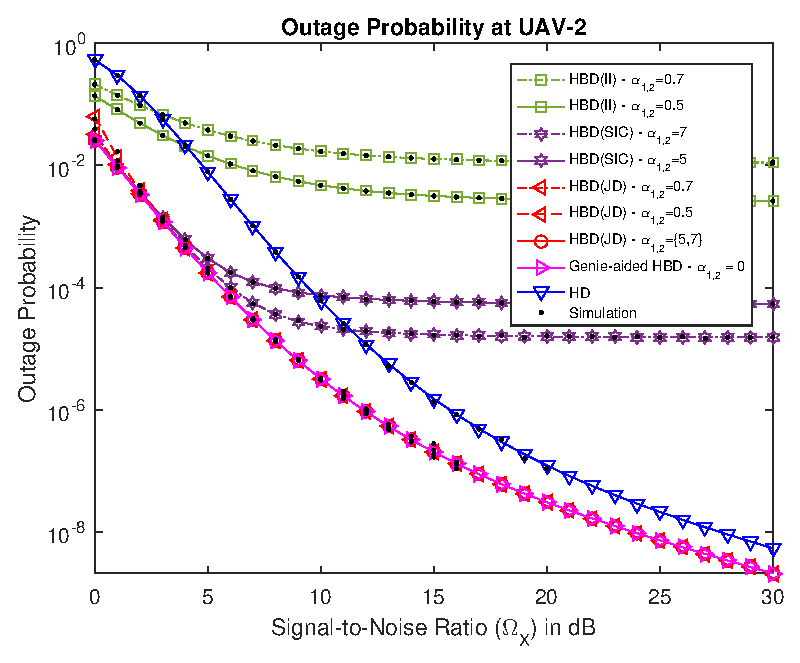
\includegraphics [width=0.45\columnwidth]{chap4_fig/fixed_pout_as2.eps}
\label{fig:JD_HBD_UCS_fixed_pout_as2}}
\hfil
\subfloat[Finite SNR diversity gain comparison at UAV-2.]{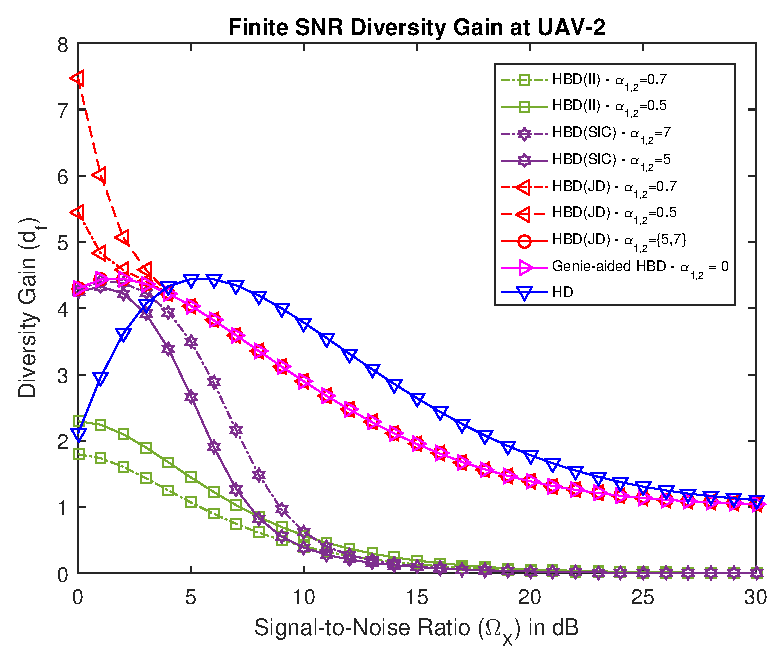
\includegraphics [width=0.45\columnwidth]{chap4_fig/fixed_df_as2.eps}
\label{fig:JD_HBD_UCS_fixed_df_as2}}
\caption{Outage probability and finite SNR diversity gain at UAV-2 (II, SIC and joint detectors) for $\alpha_{g,2}=1$.}
\label{fig:JD_HBD_UCS_fixed_as2}
\end{figure*}

The outage probabilities and diversity gains of the II, SIC, and the joint detectors are plotted in Fig. \ref{fig:JD_HBD_UCS_fixed_as2}. As a comparison, the outage probability and diversity gain of the HD-UCS are also included. From Fig. \ref{fig:JD_HBD_UCS_fixed_pout_as2}, it is observed for all inter-UAV interference levels that the joint detector achieves genie-aided outage probability at moderate and high SNR regimes. However, at very low SNR regimes, a slight performance degradation is observed for the joint detector due to weak inter-UAV interference. Additionally, it is observed that both the II and the SIC detectors are interference-limited at high SNR regimes, unlike the joint detector. Such a behavior is reflected in the intersection of the HBD-UCS outage probability with the HD-UCS in Fig. \ref{fig:JD_HBD_UCS_fixed_pout_as2}. Nonetheless, the SIC detector attains lower outage probability than the II detector under strong inter-UAV interference, e.g., $\alpha_{1,2}=5$. Similarly, the II detector attains lower outage probability than the SIC detector under weak inter-UAV interference, e.g., $\alpha_{1,2}=0.5$. 

In Fig. \ref{fig:JD_HBD_UCS_fixed_df_as2}, the diversity gain expressions of the II, SIC and the joint detectors are validated. As finite SNR diversity gain quantifies the decay of outage probability curves, it can be observed that the diversity gain of the various detectors corresponds to the steepness of the associated outage probability curves in Fig. \ref{fig:JD_HBD_UCS_fixed_pout_as2}. Furthermore, the diversity gain of the joint detector indicates that outage probability can be further improved when $\Omega_X$ is increased. It is also shown that the joint detector attains genie-aided diversity gains as $\Omega_X \to \infty$, validating Corollary \ref{JD_HBD_UCS_asymptotic_JD}. 

When compared against the HD-UCS, the joint detector achieves much better finite SNR diversity gains at low SNR regimes. However, at moderate SNR regimes, the absence of inter-UAV interference causes the HD-UCS to achieve better diversity gains than the joint detector and the genie-aided HBD-UCS. In particular, the effect of inter-UAV interference on the joint detector's finite SNR diversity gain is reflected in the second term of (\ref{JD_HBD_UCS_df_fixed_UAV2_JD}). In the case of HD-UCS, the inter-UAV interference term is absent, thus enabling better diversity gain than the joint detector. Finally, the HD-UCS, joint detector and the genie-aided HBD-UCS achieves the same diversity gains at asymptotic SNR regimes. In contrast, the diversity gain of the II and the SIC detectors approaches 0 as $\Omega_X \to \infty$ since both detectors are interference-limited at high SNR regimes. Similar to Fig. \ref{fig:JD_HBD_UCS_fixed_pout_as2}, the intersection in Fig. \ref{fig:JD_HBD_UCS_fixed_df_as2} indicates the SNR where the decay rate of the HD-UCS is greater than the HBD-UCS. However, it must be noted that a large diversity gain is not an indication of better performance in absolute terms. Instead, it only shows how fast outage probability is decaying as SNR is increasing.

%\begin{figure}[]
%\centering
%%\vspace{-0.5cm}
%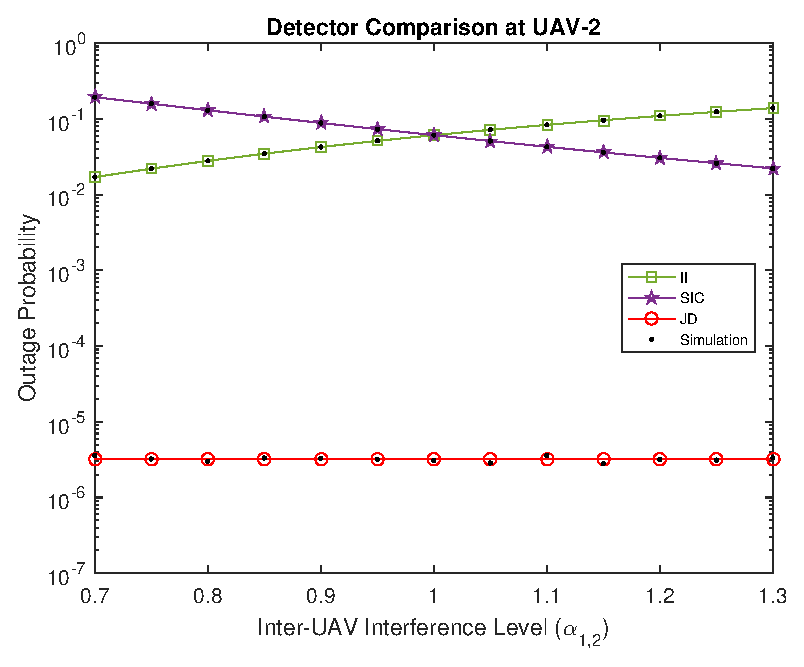
\includegraphics [width=0.9\columnwidth]{fig/fixed_det_comp_as2.eps} 
%\vspace{-0.5cm}
%\caption{Detector comparison at UAV-2 under moderate interference for $\Omega_X=10dB$ and $\alpha_{g,2}=1$.}
%\vspace{-0.5cm}
%\label{fig:fixed_det_comp_as2}
%\end{figure}

%%%%%%%%%%%%%%%%%%%%%%%%%%%%%%%%%%%%%%%%%%%%%%%%%%%%%%%%%%%%%%%%%%%%%%%%%%%%%%%%%%
% Under moderate inter-UAV interference, it can be seen that SIC detector attains lower outage probability than the II detector as inter-UAV interference ($\alpha_{1,2}$) is increased.

% When $\alpha_{1,2}=1$, i.e., the SOI and inter-UAV interference are equally strong, both the II and the SIC detectors attain similar outage probabilities.

% On the contrary, the joint detector is observed to be unaffected by inter-UAV interference and maintains a lower outage probability than the II and the SIC detectors.
%%%%%%%%%%%%%%%%%%%%%%%%%%%%%%%%%%%%%%%%%%%%%%%%%%%%%%%%%%%%%%%%%%%%%%%%%%%%%%%%%%

\begin{observation}
\emph{\emph{The impact of moderate inter-UAV interference on the joint detector is negligible, with lower outage probability observed than the II and the SIC detectors.}
}\end{observation}

It can be observed in Fig. \ref{fig:JD_HBD_UCS_fixed_pout_as2} that the SIC detector attains lower outage probability as inter-UAV interference ($\alpha_{1,2}$) is increased. Likewise, the II detector attains lower outage probability as $\alpha_{1,2}$ is decreased. On the contrary, the joint detector is observed to be unaffected by inter-UAV interference and maintains a lower outage probability than the II and the SIC detectors.

%%%%%%%%%%%%%%%%%%%%%%%%%%%%%%%%%%%%%%%%%%%%%%%%%%%%%%%%%%%%%%%%%%%%%%%%%%%%%%%%%%
% Suitable detectors for weak, moderate and strong inter-UAV interference scenarios have been identified.
%%%%%%%%%%%%%%%%%%%%%%%%%%%%%%%%%%%%%%%%%%%%%%%%%%%%%%%%%%%%%%%%%%%%%%%%%%%%%%%%%%
From Fig. \ref{fig:JD_HBD_UCS_fixed_as2}, the II and the SIC detectors are suitable for weak and strong inter-UAV interference scenarios, respectively. Furthermore, the joint detector attains, either genie-aided or near-genie-aided, outage performance over the II and the SIC detectors in weak, moderate and strong interference scenarios. Therefore, the proposed HBD-UCS with joint detector can achieve superior reliability and is suitable across weak, moderate, and strong inter-UAV interference scenarios.

\subsection{Outage and Finite SNR Diversity Gain Analysis at the System Level}

%\vspace{-0.2in}
\begin{table}[]
\centering
\caption{System Level HBD-UCS Performance Bottleneck for $\epsilon \in \{0.01, 0.001\}$}
\label{table:JD_HBD_UCS_perf_bottle}
\scalebox{0.7}{\begin{tabular}{cccc}
\hline
Mode				& $\alpha_{1,2}$ 									& $Pr\big(\mathcal{O}_{gs}\big) \leq Pr\big(\mathcal{O}_{2}\big)$ & $Pr\big(\mathcal{O}_{gs}\big) > Pr\big(\mathcal{O}_{2}\big)$ \\ \hline \hline
 $HBD(II)$	& $\alpha_{1,2} \in \{0.5, 0.7\}$ & $0dB \leq \Omega_X \leq 30dB$ & - \\ 
 $HBD(SIC)$ & $\alpha_{1,2} = 5 $  						& $4dB < \Omega_X \leq 30dB$ 	  & $0dB \leq \Omega_X \leq 4dB$ \\
 $HBD(SIC)$ & $\alpha_{1,2} = 7 $ 						& $7dB < \Omega_X \leq 30dB$ 		& $0dB \leq \Omega_X \leq 7dB$ \\ 
 $HBD(JD)$  & $\alpha_{1,2} \in \{0.5, 0.7\}$ & $0dB \leq \Omega_X < 2dB$  		& $2dB \leq \Omega_X \leq 30dB$ \\
 $HBD(JD)$  & $\alpha_{1,2} \in \{5, 7\}$ 		& - 														& $0dB \leq \Omega_X \leq 30dB$ \\ \hline
\end{tabular}}
\end{table}

\begin{figure*}[]
\centering
\subfloat[System level outage probability comparison.]{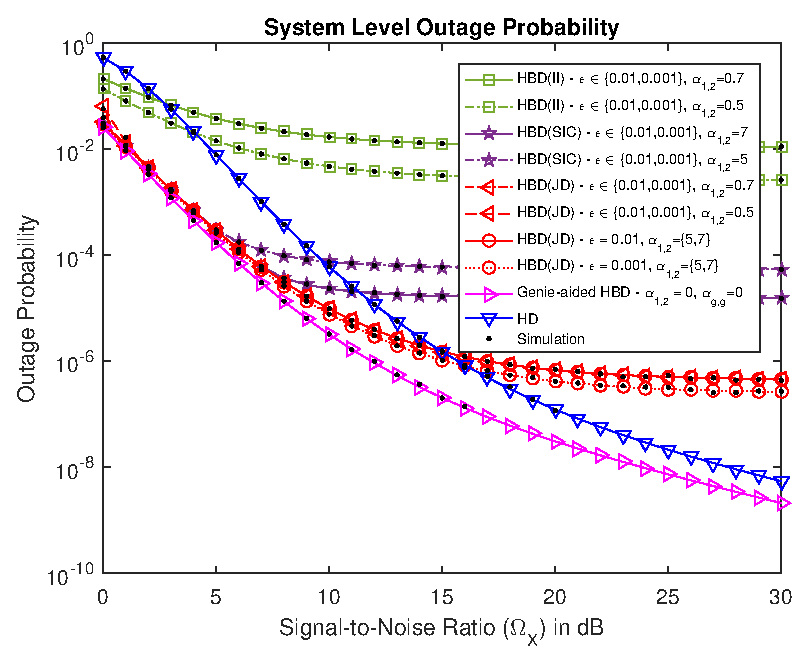
\includegraphics [width=0.45\columnwidth]{chap4_fig/fixed_pout_sys.eps}
\label{fig:JD_HBD_UCS_fixed_pout_sys}}
\hfil
\subfloat[System level finite SNR diversity gain comparison.]{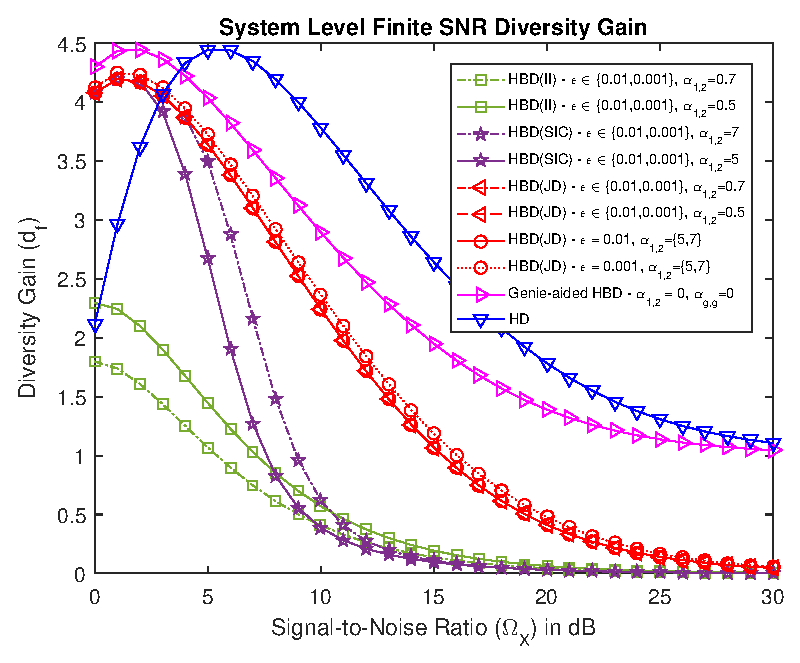
\includegraphics [width=0.45\columnwidth]{chap4_fig/fixed_df_sys.eps}
\label{fig:JD_HBD_UCS_fixed_df_sys}}
\caption{System level outage probability and finite SNR diversity gain (II, SIC and joint detectors) for $\alpha_{g,2}=1$, $\alpha_{g,g}=1$, $\gamma_{\phi}^2=-130dBm$ and $\epsilon\in\{0.01, 0.001\}$.}
\label{fig:JD_HBD_UCS_fixed_sys_lvl}
\end{figure*}
%%%%%%%%%%%%%%%%%%%%%%%%%%%%%%%%%%%%%%%%%%%%%%%%%%%%%%%%%%%%%%%%%%%%%%%%%%%%%%%%%%
% When the II detector is used, the system level performance (outage probability and diversity gain) of the HBD-UCS is constrained by inter-UAV interference.

% For the SIC detector, the system level performance of the HBD-UCS at low SNR regime is noise-limited. Residual SI is also treated as noise at the FD-enabled GS. Therefore, the GS is the bottleneck at low SNR regimes. When SNR is high, the system level performance is constrained by the inter-UAV interference at UAV-2.

% For JD, the system level performance of the HBD-UCS is observed to be constrained by residual SI under strong inter-UAV interference ($\alpha_{1,2} \in \{5,7\}$). For weak inter-UAV interference, e.g., $\alpha_{1,2} \in \{0.5,0.7\}$, system level performance is only constrained by $\alpha_{1,2}$ at very low SNR regimes.

% When compared against the II and the SIC detectors, the joint detector enables the HBD-UCS to achieve near-genie-aided system level performance at low SNR regimes under moderate and strong inter-UAV interference.

% These observations are validated through numerical simulations and tabluted in Table \ref{table:perf_bottle}.
%%%%%%%%%%%%%%%%%%%%%%%%%%%%%%%%%%%%%%%%%%%%%%%%%%%%%%%%%%%%%%%%%%%%%%%%%%%%%%%%%%

\begin{observation}
\emph{\emph{At the system level, the HBD-UCS with JD achieves near-genie-aided performance at low SNR regimes. In contrast, SI causes the HBD-UCS with JD to be suboptimal at moderate and high SNR regimes.}
}\end{observation}

The system level outage probability and diversity gain are plotted in Fig. \ref{fig:JD_HBD_UCS_fixed_sys_lvl} for the HBD-UCS and the HD-UCS. When the II detector is used, the system level performance (outage probability and diversity gain) of the HBD-UCS is constrained by inter-UAV interference. For the SIC detector, the system level performance of the HBD-UCS at low SNR regime is noise-limited. Residual SI is also treated as noise at the FD-enabled GS. Therefore, the GS is the bottleneck at low SNR regimes. When SNR is high, the system level performance is constrained by the inter-UAV interference at UAV-2. For JD, the system level performance of the HBD-UCS is observed to be constrained by residual SI under strong inter-UAV interference ($\alpha_{1,2} \in \{5,7\}$). For weak inter-UAV interference, e.g., $\alpha_{1,2} \in \{0.5,0.7\}$, system level performance is only constrained by $\alpha_{1,2}$ at very low SNR regimes. 

%%%%%%%%%%%%%%%%%%%%%%%%%%%%%%%%%%%%%%%%%%%%%%%%%%%%%%%%%%%%%%%%%%%%%%%%%%%%%%%%%%
% HBD-UCS with JD achieves near-genie-aided system level performance
%%%%%%%%%%%%%%%%%%%%%%%%%%%%%%%%%%%%%%%%%%%%%%%%%%%%%%%%%%%%%%%%%%%%%%%%%%%%%%%%%%

When compared against the II and the SIC detectors, the joint detector enables the HBD-UCS to achieve near-genie-aided system level performance at low SNR regimes under weak, moderate and strong inter-UAV interference levels. \textcolor{black}{However, the advantages of the joint detector comes at the cost of higher computational complexity.} These observations are validated through numerical simulations and tabulated in Table \ref{table:JD_HBD_UCS_perf_bottle}.

\subsection{Finite SNR DMT Analysis at UAV-2 and System level}

\begin{figure*}[]
\centering
\subfloat[Finite SNR DMT at UAV-2.]{\includegraphics [width=0.45\columnwidth]{chap4_fig/var_df_as2.eps}
\label{fig:JD_HBD_UCS_var_df_as2}}
\hfil
\subfloat[System level finite SNR DMT.]{\includegraphics [width=0.45\columnwidth]{chap4_fig/var_df_sys.eps}
\label{fig:JD_HBD_UCS_var_df_sys_lvl}}
\caption{Finite SNR DMT at UAV-2 and system level (II, SIC and joint detectors) for $\alpha_{g,2}=1$, $\alpha_{g,g}=1$, $\gamma_{\phi}^2=-130dBm$ and $\Omega_X=10dB$.}
\label{fig:JD_HBD_UCS_var_jd}
%\vspace{-0.5cm}
\end{figure*}
%%%%%%%%%%%%%%%%%%%%%%%%%%%%%%%%%%%%%%%%%%%%%%%%%%%%%%%%%%%%%%%%%%%%%%%%%%%%%%%%%%
% For Fig 6a:
% At low multiplexing gains, the joint detector at UAV-2 attains genie-aided finite SNR diversity gains. At high multiplexing, the joint detector attains near-genie-aided finite SNR diversity gains as inter-UAV interference increases. 

% On the other hand, the II and the SIC detectors at UAV-2 is observed to attain lower finite SNR diversity gains than the HD-UCS at low multiplexing gains. Furthermore, only the SIC detector showed better finite SNR diversity gains than the HD-UCS at moderate multiplexing gains, e.g., $0.45 \leq r_f \leq 0.6$.

% Finally, it is observed that the HD-UCS can only achieve non-zero diversity gain only up to $r_f = 0.5$ while the joint detector achieves non-zero diversity gains up to twice that of the HD-UCS. 
%%%%%%%%%%%%%%%%%%%%%%%%%%%%%%%%%%%%%%%%%%%%%%%%%%%%%%%%%%%%%%%%%%%%%%%%%%%%%%%%%%
% For Fig 6b:
% At the system level, the finite SNR diversity gain is constrained by residual SI at the fd-enabled GS due to imperfect SI channel estimation ($\epsilon$) for the II, SIC, and the joint detectors.

% Only the SIC and the joint detectors exhibited better finite SNR diversity gains than the HD-UCS as inter-UAV interference increases for  $0.45 \leq r_f \leq 0.65$.
%%%%%%%%%%%%%%%%%%%%%%%%%%%%%%%%%%%%%%%%%%%%%%%%%%%%%%%%%%%%%%%%%%%%%%%%%%%%%%%%%%

For variable transmission rate schemes, finite SNR DMT curves at UAV-2 are presented in Fig. \ref{fig:JD_HBD_UCS_var_df_as2}. At the system level, the HBD finite SNR DMT is plotted in Fig. \ref{fig:JD_HBD_UCS_var_df_sys_lvl}.

\begin{observation}
\emph{\emph{As inter-UAV interference increases, the joint detector attains better diversity gain at higher multiplexing gains than the II detector, SIC detector, and HD-UCS at both UAV-2 and system level.}
}\end{observation}

In Fig. \ref{fig:JD_HBD_UCS_var_df_as2}, it is shown that the joint detector at UAV-2 attains genie-aided finite SNR diversity gains at low multiplexing gains. At high multiplexing gains, the joint detector attains near-genie-aided finite SNR diversity gains as inter-UAV interference increases. On the other hand, the II and the SIC detectors at UAV-2 are observed to attain lower finite SNR diversity gains than the HD-UCS at low multiplexing gains. Furthermore, only the SIC detector showed better finite SNR diversity gains than the HD-UCS at moderate multiplexing gains, e.g., $0.45 \leq r_f \leq 0.6$. Finally, it is observed that the HD-UCS achieves non-zero diversity gain only up to $r_f = 0.5$ while the joint detector achieves non-zero diversity gains up to twice that of the HD-UCS. 

At the system level (Fig. \ref{fig:JD_HBD_UCS_var_df_sys_lvl}), the finite SNR diversity gain is constrained by residual SI at the FD-enabled GS due to imperfect SI channel estimation ($\epsilon$) for the II, SIC, and the joint detectors. Only the SIC and the joint detectors exhibited better finite SNR diversity gains than the HD-UCS as inter-UAV interference increases for  $0.45 \leq r_f \leq 0.65$.

%%%%%%%%%%%%%%%%%%%%%%%%%%%%%%%%%%%%%%%%%%%%%%%%%%%%%%%%%%%%%%%%%%%%%%%%%%%%%%%%%%
% The joint detector enables HBD-UCS to achieve better reliability and higher throughput than existing HD-UCS in multi-UAV networks
%%%%%%%%%%%%%%%%%%%%%%%%%%%%%%%%%%%%%%%%%%%%%%%%%%%%%%%%%%%%%%%%%%%%%%%%%%%%%%%%%%
From Fig. \ref{fig:JD_HBD_UCS_var_jd}, the joint detector enables HBD-UCS to achieve better reliability in multi-UAV networks while attaining higher throughput than existing HD-UCS.

\subsection{Finite SNR Multiplexing Gain Regions at UAV-2}

\begin{figure*}[]
\centering
\subfloat[SIC detector.]{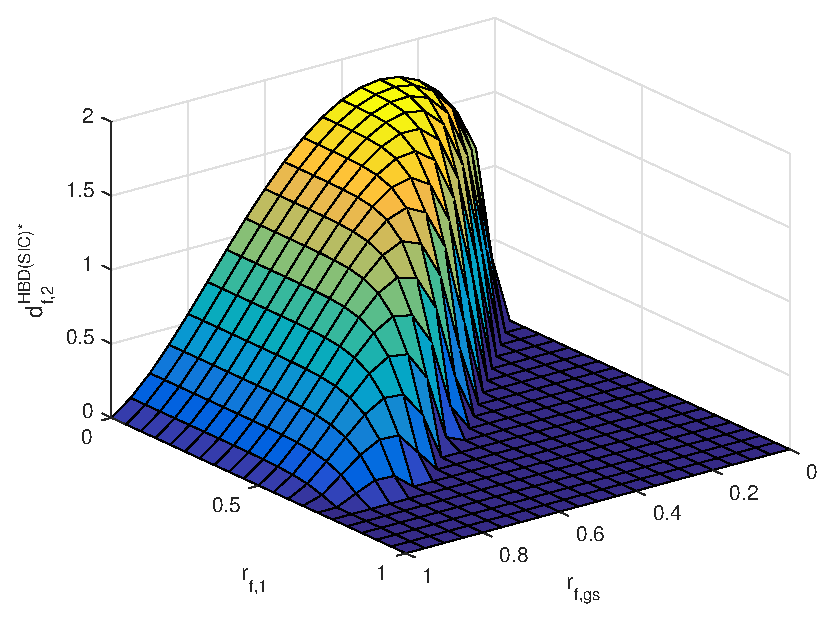
\includegraphics [width=0.45\columnwidth]{chap4_fig/var_df_uav2_sic_surf.eps}
\label{fig:JD_HBD_UCS_var_df_uav2_sic_surf}}
\hfil
\subfloat[Joint detector.]{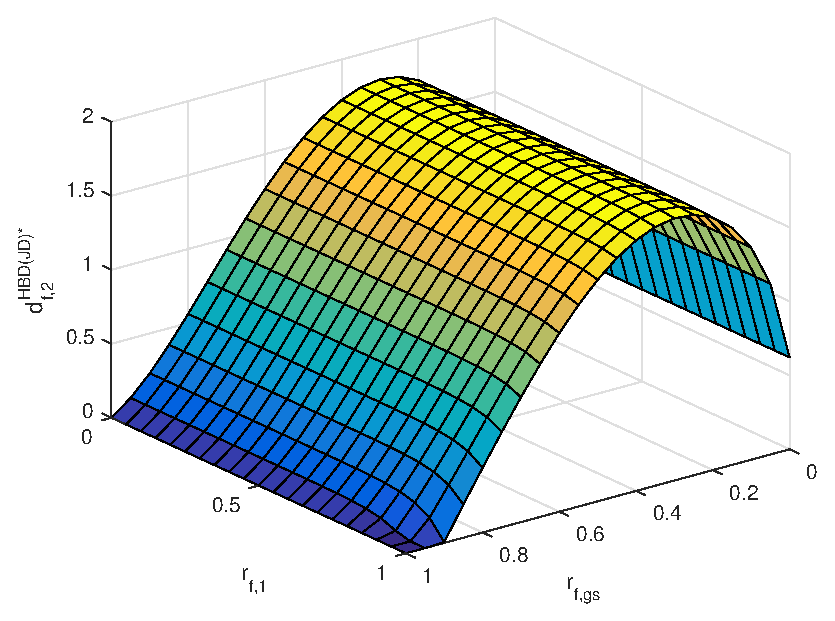
\includegraphics [width=0.45\columnwidth]{chap4_fig/var_df_uav2_jd_surf.eps}
\label{fig:JD_HBD_UCS_var_df_uav2_jd_surf}}
\caption{Achievable finite SNR diversity gain of the SIC detector and joint detector at UAV-2 for different multiplexing gains at UAV-1 ($r_{f,1}$) and the GS ($r_{f,gs}$) when $\alpha_{g,2}=1$, $\alpha_{1,2}=15$ and $\Omega_X=10dB$.}
\label{fig:JD_HBD_UCS_var_mgr_surf_uav2}
%\vspace{-0.5cm}
\end{figure*}

%%%%%%%%%%%%%%%%%%%%%%%%%%%%%%%%%%%%%%%%%%%%%%%%%%%%%%%%%%%%%%%%%
% The SIC detector achieves non-zero diversity gain when the multiplexing gain of the SOI is larger than the multiplexing gain of the interferer. 
% On the contrary, the achievable diversity gain of the joint detector is independent of the multiplexing gain of the interferer.
%%%%%%%%%%%%%%%%%%%%%%%%%%%%%%%%%%%%%%%%%%%%%%%%%%%%%%%%%%%%%%%%%

\begin{figure*}[]
\centering
\subfloat[II and joint detector, $\alpha_{1,2}=0.1$.]{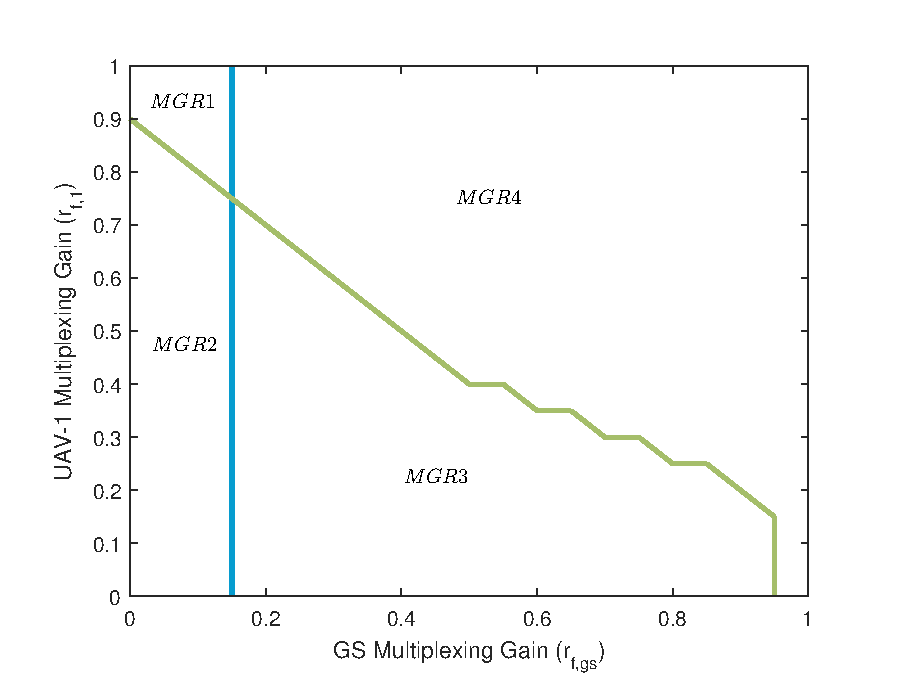
\includegraphics [width=0.45\columnwidth]{chap4_fig/var_df_uav2_jd_ii_mgr_annot2.eps}
\label{fig:JD_HBD_UCS_var_df_uav2_jd_ii_mgr_annot}}
\hfil
\subfloat[SIC and joint detector, $\alpha_{1,2}=15$.]{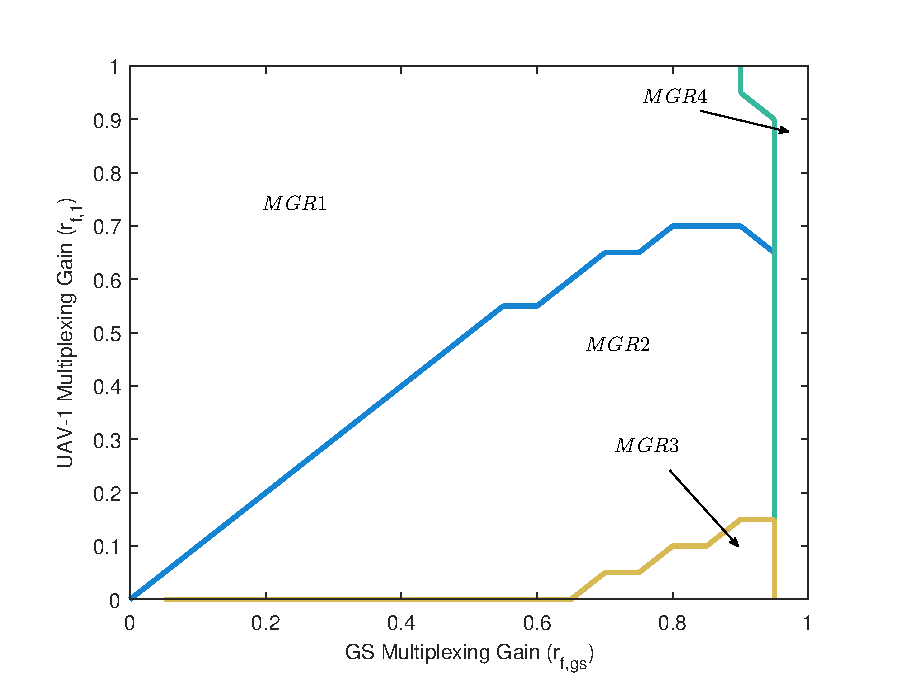
\includegraphics [width=0.45\columnwidth]{chap4_fig/var_df_uav2_jd_sic_mgr_annot2.eps}
\label{fig:JD_HBD_UCS_var_df_uav2_jd_sic_mgr_annot}}
\caption{Overlapping finite SNR MGRs of the II, SIC and joint detectors at UAV-2 for $\alpha_{g,2}=1$, $\alpha_{1,2}=\{0.1,15\}$ and $\Omega_X=10dB$. (The MGR separation can be smoothen by plotting the regions with very high resolutions.)}
\label{fig:JD_HBD_UCS_var_mgr_uav2}
%\vspace{-0.5cm}
\end{figure*}

%%%%%%%%%%%%%%%%%%%%%%%%%%%%%%%%%%%%%%%%%%%%%%%%%%%%%%%%%%%%%%%%%
% The joint detector achieves non-zero finite SNR diversity gains over a larger MGR region than the II detector, with $d_{f,2}^{HBD(JD)*} > d_{f,2}^{HBD(II)*}$ in $MGR2$.

% Similarly, the joint detector achieves non-zero finite SNR diversity gains over a larger MGR region than the SIC detector. Furthermore, $d_{f,2}^{HBD(JD)*} > d_{f,2}^{HBD(SIC)*}$ in $MGR2$. However, $d_{f,2}^{HBD(JD)*} = d_{f,2}^{HBD(II)*}$ in $MGR3$ when $r_{f,gs}$ is high and $r_{f,1}$ is low since the SIC detector is more likely to detect and remove $x_{1}[t]$.

% As inter-UAV interference increases, the joint detector can achieve non-zero diversity gain over a large MGR. In other words, the interfering signal can be transmitted at higher data rates as inter-UAV interference increases. 
%%%%%%%%%%%%%%%%%%%%%%%%%%%%%%%%%%%%%%%%%%%%%%%%%%%%%%%%%%%%%%%%%

So far, we have assumed that the multiplexing gains of the FD-enabled GS and UAV-1 are the same, i.e., $r_{f,1}=r_{f,gs}=r_f$. In contrast, we assume different multiplexing gains for UAV-1 and the GS in the subsequent analysis. The achievable finite SNR diversity gains for the SIC detector $\big(d_{f,2}^{HBD(SIC)*}\big)$ and the joint detector $\big(d_{f,2}^{HBD(JD)*}\big)$ are plotted in Fig. \ref{fig:JD_HBD_UCS_var_df_uav2_sic_surf} and Fig. \ref{fig:JD_HBD_UCS_var_df_uav2_jd_surf}, respectively. We omit plotting the achievable finite SNR diversity gain of the II detector $\big(d_{f,2}^{HBD(II)*}\big)$ as the expression is independent of the multiplexing gain of the interference ($r_{f,1}$).

\begin{observation}
\emph{\emph{The SIC detector achieves non-zero diversity gain when the multiplexing gain of the SOI is larger than the multiplexing gain of the interferer. On the contrary, the achievable diversity gain of the joint detector is independent of the multiplexing gain of the interferer.}
}\end{observation}

From Fig. \ref{fig:JD_HBD_UCS_var_mgr_surf_uav2}, it is observed that the SIC detector achieves non-zero diversity gain when the multiplexing gain of the SOI is larger than the multiplexing gain of the interferer. As noted in \cite{narasimhan2006finite}, the multiplexing gain of a variable transmission rate scheme determines the impact of Rician $K$ factors on outage decay. In particular, a higher multiplexing gain elicits a stronger influencing effect of the Rician $K$ factor on outage decay and vice versa. The same principle also explains the trend seen in Fig. \ref{fig:JD_HBD_UCS_var_df_uav2_sic_surf} for the SIC detector. As $r_{f,1}$ increases, the Rician $K$ factor corresponding to the interfering link ($K_{Y_1}$) starts to affect the overall outage decay of the SIC detector. Therefore, $r_{f,gs}$ must also increase , i.e., $0<r_{f,1}<r_{f,gs}<1$ to offset the influence of $K_{Y_1}$ on the overall outage decay with the Rician $K$ factor corresponding to the SOI link ($K_{X_{gs}}$).

On the contrary, Fig. \ref{fig:JD_HBD_UCS_var_df_uav2_jd_surf} shows that the achievable diversity gain of the joint detector is independent of the multiplexing gain of the interferer. Therefore, non-zero $d_{f,2}^{HBD(JD)*}$ can be obtained for a wider range of $r_{f,1}$ and $r_{f,gs}$ values compared to the SIC detector. In strong inter-UAV interference scenarios, the joint detector enables the proposed HBD-UCS to accommodate a wider range of data rate requirements compared to the SIC detector. For instance, video streaming capabilities can be deployed on UAV-1 while still meeting the QoS requirements of CNPC links at the FD-enabled GS, even when inter-UAV interference is strong. Hence JD-based HBD-UCS deployment in UAV networks is attractive when the high data rate requirements are met, albeit at the cost of higher computational complexity compared to SIC-based HBD-UCS\footnote{The complexity of the joint detector depends on the particular encoding scheme (e.g., Low-density parity-check or turbo codes) and decoding scheme (e.g., bipartite graph-based or trellis-based decoders), interested readers can refer to \cite{shubhi2017joint} for more details}.
 \newpage
\begin{observation}
\emph{\emph{The joint detector achieves non-zero diversity gain over a larger multiplexing gain region than the II and the SIC detectors under equivalent inter-UAV interference levels.}
}\end{observation}

In Fig. \ref{fig:JD_HBD_UCS_var_df_uav2_jd_ii_mgr_annot}, the MGRs of the joint detector and II detector are shown for $\alpha_{1,2}=0.1$. In particular, the joint detector achieves non-zero $d_{f,2}^{HBD(JD)*}$ in regions $MGR2$ and $MGR3$ while the II detector achieves non-zero $d_{f,2}^{HBD(II)*}$ in regions $MGR1$ and $MGR2$. In $MGR4$, both the joint detector and II detector achieve zero finite SNR diversity gains. Evidently, the joint detector achieves non-zero finite SNR diversity gains over a larger MGR region than the II detector, with $d_{f,2}^{HBD(JD)*} > d_{f,2}^{HBD(II)*}$ in $MGR2$.

In Fig. \ref{fig:JD_HBD_UCS_var_df_uav2_jd_sic_mgr_annot}, the MGRs of the joint detector and SIC detector are shown for $\alpha_{1,2}=15$. The joint detector achieves non-zero $d_{f,2}^{HBD(JD)*}$ in regions $MGR1$, $MGR2$ and $MGR3$. The SIC detector achieves non-zero $d_{f,2}^{HBD(SIC)*}$ in regions $MGR2$ and $MGR3$. In $MGR4$, both the joint detector and SIC detector achieve zero finite SNR diversity gains. 

From Fig. \ref{fig:JD_HBD_UCS_var_df_uav2_jd_sic_mgr_annot}, it can be observed that the joint detector achieves non-zero finite SNR diversity gains over a larger MGR region than the SIC detector. Furthermore, $d_{f,2}^{HBD(JD)*} > d_{f,2}^{HBD(SIC)*}$ in $MGR2$. However, $d_{f,2}^{HBD(JD)*} = d_{f,2}^{HBD(II)*}$ in $MGR3$ when $r_{f,gs}$ is high and $r_{f,1}$ is low since the SIC detector is more likely to detect and remove $x_{1}[t]$. As inter-UAV interference increases, the joint detector can achieve non-zero diversity gain over a large MGR. In other words, the interfering signal can be transmitted at higher data rates as inter-UAV interference increases. 

The trends in Fig. \ref{fig:JD_HBD_UCS_var_mgr_surf_uav2} and Fig. \ref{fig:JD_HBD_UCS_var_mgr_uav2} show that the joint detector enables the proposed HBD-UCS to achieve higher reliability than the II and SIC detectors while meeting a wider range of QoS requirements. Therefore, the JD-based HBD-UCS is more flexible in responding to changing QoS requirements and exhibits better reliability over II-based and SIC-based HBD-UCS in multi-UAV networks.

%%%%%%%%%%%%%%%%%%%%%%%%%%%%%%%%%%%%%%%%%%%%%%%%%%%%%%%%%%%%%%%%%%%%%%%%%%%%%%%%%%%%%%%%%%%%%%%%%%%%%%%%%%%%%%%%%%%%%%%%%%%%%%%%%%%%%%%%%
% Section: Conclusion
\section{Chapter Summary}
An HBD-UCS with JD is proposed in this chapter as a step towards addressing spectrum scarcity in UAV communications. An innovative approach to deriving closed-form outage probability and finite SNR diversity gain expressions over Rician fading channels is also presented. Through a comprehensive performance analysis, suitable detectors for various inter-UAV interference scenarios are identified. The degree of performance improvements offered by the joint detector over the II and the SIC detectors are also highlighted. It is also observed that the SIC detector achieves non-zero diversity gain when the interfering signal from UAV-1 is transmitted at a lower data rate than the SOI from the FD-enabled GS. However, when inter-UAV interference is sufficiently strong, the joint detector is observed to be independent of the data rate of the interfering signal. An analysis of the MGR for the II, SIC, and the joint detectors is also conducted, where it is shown that the JD-based HBD-UCS can support a wide range of data rate requirements while achieving superior reliability over the II-based and SIC-based HBD-UCS. 

% Work is in progress on evaluating the JD-based HBD-UCS against II-based HBD-UCS, SIC-based HBD-UCS and HD-UCS through stochastic geometry framework. In addition, the impact of Rician $K$ factors on HBD-UCS performance, extending the outage and finite SNR analysis framework for combinations of Rician and Rayleigh fading with imperfect channel estimation, the design of robust and low complexity SIC detectors and joint detectors that considers multiple UAVs and FD-enabled GSs, and beamforming solutions are also being investigated as part of future works.

While II-based, SIC-based, and JD-based HBD-UCSs has been shown to be highly effective for UAV communications over Rician fading channels, the performance of joint detection over channels experiencing joint fading and shadowing is unclear. Thus, in the next chapter, the performance of the HBD-UCS is evaluated in a Rician shadowed fading environment to understand the effects of fading and shadowing on UAV communications.


